\documentclass[a4paper,12pt,oneside,openright]{report}
% \documentclass[a4paper,12pt,twoside,openright]{report}

\usepackage{cmap}
\usepackage[english]{babel}
\usepackage[utf8]{inputenc}
\usepackage[T1]{fontenc}
\usepackage{lmodern}
\usepackage{microtype}
\usepackage{setspace}

\usepackage[a4paper,
            bindingoffset=0.5cm,
            top=2.5cm,
            bottom=2.5cm,
            left=2.5cm,
            right=2.5cm,
            marginparwidth=2.0cm]{geometry}

\usepackage{amsmath}
\usepackage{amssymb}
\usepackage{amsthm}
\usepackage{array}
\usepackage{caption}
\usepackage{changepage}
\usepackage{enumitem}
\usepackage{float}
\usepackage{graphicx}
\usepackage[bookmarks,pdfusetitle,unicode]{hyperref}
\usepackage[none]{hyphenat}  % turn off hyphenation (words splitting)
\usepackage{indentfirst}
\usepackage{lipsum}
\usepackage[newfloat]{minted}
\usepackage[all,defaultlines=3]{nowidow}  % prevent single lines between pages
\usepackage{physics}
\usepackage{showlabels}  % TODO comment/remove at the end
\usepackage{siunitx}
\usepackage{tikz}
\usepackage[colorinlistoftodos,textsize=tiny]{todonotes}

% dots in the table of contents
\usepackage{tocloft}
\renewcommand{\cftchapdotsep}{\cftdotsep}

% headers customization
\usepackage{fancyhdr}
\pagestyle{fancy}
\fancyhf{}  % clear all current header and footer fields

\renewcommand{\headrulewidth}{1.0pt}
\renewcommand{\chaptermark}[1]{\markboth{\MakeUppercase{\thechapter.~#1}}{}}
\fancyhead[LE,RO]{\bfseries\thepage}  % page number: left on even, right on odd
\fancyhead[RE]{\bfseries\nouppercase{\leftmark}\chaptermark}  % right on even
\fancyhead[LO]{\bfseries\nouppercase{\rightmark}\sectionmark}  % left on odd

\fancypagestyle{plain}{% plain = e.g. clear pages and where chapters begin
    \fancyhf{}
    \fancyhead[RO]{\bfseries\thepage}
    % \renewcommand{\headrulewidth}{0pt}
}

% footnotes customization
\setlength{\footnotesep}{10pt}

\renewcommand{\footnoterule}{
    \kern 12pt
    \hrule width \textwidth height 0.4pt
    \kern 5pt
}

\interfootnotelinepenalty=10000  % do not split between pages

% do not reset footnote counter between chapters
\usepackage{chngcntr}
\counterwithout{footnote}{chapter}

% captions customization
\captionsetup{justification=centering}

% dotted borders around links in PDF viewers
\hypersetup{pdfborderstyle=/S/D/D[3 2]/W 0.25,pdfborder=0 0 1}

% no borders around links in PDF viewers
% \hypersetup{colorlinks,allcolors=black}

% miscellaneous and additional text formatting
\setstretch{1.25}
\setlength{\parskip}{0.75em}
\setlength{\headheight}{15pt}
\addtolength{\topmargin}{-3pt}

\setminted{fontsize=\small,baselinestretch=1}


%
% Metadata
%
\title{Klasyfikacja z grupą otwartą w danych wysokowymiarowych}
\author{Szymon Tomasz Datko}
\date{2024}

% \def\TheUniversity{Politechnika Wrocławska}
\def\TheUniversity{Wrocław University of Science and Technology}
% \def\TheFaculty{Wydział Informatyki i Telekomunikacji}
\def\TheFaculty{Faculty of Information and Communication Technology}
% \def\TheHeader{Rozprawka Doktorska}
\def\TheHeader{Doctoral Thesis}

\def\TheTitleEN{Open-set classification \\
                in high-dimensional data.}
\def\TheTitlePL{Klasyfikacja z grupą otwartą \\
                w danych wysokowymiarowych.}

\def\TheAuthorLabel{Author}
% \def\TheAuthorTitle{mgr inż.}
\def\TheAuthorTitle{MSc Eng}
\def\TheAuthorName{Szymon Tomasz Datko}

\def\TheSupervisorLabel{Supervisor}
% \def\TheSupervisorTitle{dr hab. inż.}
\def\TheSupervisorTitle{Prof PhD Eng}
\def\TheSupervisorName{Henryk Maciejewski}

\def\TheDate{Wrocław 2024}

\def\TheSentenceText{We don't make mistakes; \\
                     we just have happy accidents.}
\def\TheSentenceAuthor{Bob Ross}


%
% Content
%
\begin{document}
    {%
        \pagestyle{empty}

        \begin{titlepage}
    \thispagestyle{empty}
    \pagenumbering{gobble}  % do not set page number
    \pdfbookmark{Title page}{title-page}
    \setlength{\parskip}{0em}
    \setstretch{1.25}

    \begin{center}
        \Large
        \scshape

        \TheUniversity
    \end{center}

    \vspace{-2.0em}

    \begin{center}
        \large
        \scshape

        \TheFaculty
    \end{center}

    \hrule
    \vfill

    \begin{center}
        \huge
        \bfseries

        \TheHeader
    \end{center}

    \vfill

    \hfill
    \begin{minipage}[t]{0.6\textwidth}
        \begin{center}
            \Large

            \TheTitleEN
        \end{center}

        \vspace{1.0em}

        \begin{center}
            \TheTitlePL
        \end{center}
    \end{minipage}

    \vfill

    \hfill
    \begin{minipage}[t]{0.6\textwidth}
        \large
        \underline{\TheAuthorLabel}: \\
        \vspace{0.25em}
        {\small \TheAuthorTitle}
        \TheAuthorName
    \end{minipage}

    \vfill

    \hfill
    \begin{minipage}[t]{0.6\textwidth}
        \large
        \underline{\TheSupervisorLabel}: \\
        \vspace{0.25em}
        {\small \TheSupervisorTitle}
        \TheSupervisorName
    \end{minipage}

    \vfill
    \vfill
    \hrule

    \begin{center}
        \large
        \scshape

        \TheDate
    \end{center}
\end{titlepage}

        \cleardoublepage

        \null  % there must be something before the vfill
\vfill
\vfill
\vfill
\vfill
\vfill

\hfill
\begin{minipage}[t]{0.4\textwidth}
    \setstretch{1.5}
    \normalsize
    \itshape

    ,,\TheSentenceText''

    \vspace{0.25\baselineskip}
    \hfill
    – \TheSentenceAuthor
\end{minipage}

\vfill

        \cleardoublepage
    }


    \pagenumbering{roman}
    \setcounter{page}{1}

    \phantomsection  % so hyperref links will lead to the correct place in document
\addcontentsline{toc}{chapter}{Abstract}

\chapter*{Abstract}
\label{chapter:abstract}

\todo{Do zrobienia}  % TODO
.


\section*{Keywords}
\label{section:keywords}

\begin{itemize}
    \item[–] Open-Set Classification.
    \item[–] Out-of-Distribution Detection.
    \item[–] Measures of Outlierness.
    \item[–] High-Dimensional Feature Vectors.
    \item[–] Data Representation Techniques.
\end{itemize}

    \cleardoublepage

    \phantomsection  % so hyperref links will lead to the correct place in document
\addcontentsline{toc}{chapter}{Streszczenie}

\chapter*{Streszczenie}
\label{chapter:streszczenie}

\todo{Do zrobienia}  % TODO
\lipsum[1]


\section*{Słowa kluczowe}
\label{section:slowa-kluczowe}

\begin{itemize}
    \item[–] A,
    \item[–] B,
    \item[–] C,
\end{itemize}

    \cleardoublepage

    \phantomsection  % so hyperref links will lead to the correct place in document
\addcontentsline{toc}{chapter}{Acknowledgments}

\chapter*{Acknowledgments}
\label{chapter:acknowledgments}

\todo{Do zrobienia}  % TODO
\lipsum[1]

    \cleardoublepage


    \pagenumbering{arabic}
    \setcounter{page}{1}

    \phantomsection  % so hyperref links will lead to the correct place in document
\addcontentsline{toc}{chapter}{\contentsname}

\tableofcontents

    \cleardoublepage

    \chapter{Introduction}
\label{chapter:introduction}

\todo{Do zrobienia}  % TODO
\lipsum[1]


\section{Motivation – problem formulation}
\label{section:motivation}

\todo{Do zrobienia}  % TODO
\lipsum[1]


\section{Main contributions of this work}
\label{section:contributions}

\todo{Do zrobienia}  % TODO
\lipsum[1]


\section{Document organisation}
\label{section:document-organisation}

\todo{Do zrobienia}  % TODO
\lipsum[1]

    \cleardoublepage

    \chapter{Related work}
\label{chapter:related-work}

\todo{Do zrobienia}  % TODO
\lipsum[1]


\section{Explainability and trustworthiness}
\label{section:trustworthiness}

\todo{Do zrobienia}  % TODO
\lipsum[1]


\section{Open-set classification}
\label{section:contributions}

\todo{Do zrobienia}  % TODO
\lipsum[1]


\section{Measures of outlierness}
\label{section:measures}

\todo{Do zrobienia}  % TODO
\lipsum[1]


\subsection{Angle-Based Outlier Factor}
\label{section:abof}

\todo{Do zrobienia}  % TODO
\lipsum[1]


\subsection{Integrated Rank Weighted Depth}
\label{section:irwd}

\todo{Do zrobienia}  % TODO
\lipsum[1]


\subsection{Local Outlier Factor}
\label{section:lof}

\todo{Do zrobienia}  % TODO
\lipsum[1]

    \cleardoublepage

    \chapter{Simulations}
\label{chapter:simulations}

\todo{Do zrobienia}  % TODO
\lipsum[1]


\section{Experiments organisation}
\label{section:experiments}

\todo{Do zrobienia}  % TODO
\lipsum[1]


    \cleardoublepage

    \chapter{Performance of OOD detectors in~image and text recognition tasks}
\label{chapter:real-data}

In this chapter the results of research conducted on image data and text documents are presented. The performance of popular outlier detection methods is shown when applied to feature spaces generated by various Deep Learning (DL) models. It is shown that the effectiveness of OOD detectors are significantly impacted by the characteristics of the feature spaces generated by deep learning representation techniques. Hence, the~extended way of evaluating the OOD-generalization properties for selected DL-based data representation methods is proposed. The results are introduced as comparison with traditional measures of efficiency, as being used in current literature. In addition, the differences in properties of the feature vectors obtained from various representation techniques are discussed, resulting in a~number of recommendations on the OOD detectors selection.

The described results are base and motivation for further, dedicated publication \cite{Datko-2024} that was prepared and submitted at the same time as this dissertation chapter.

\cleardoublepage{}


\section{Data sources and experiment organization}
\label{section:real-organization}

During the research, the performance of OOD measures in the OOD detection benchmarks was analyzed, involving both image data and text documents as inputs.

For image data, the ImageNet-1K \cite{Deng-2009} dataset was selected as the in-distribution (ID) data, containing 1`281`167 training samples in total, divided into $m = 1000$ classes (i.e., roughly 1300 samples per class). The following datasets were utilized as the source of out-of-distribution (OOD) samples:
\vspace{-0.5\baselineskip}
\begin{itemize}
    \item ImageNet-O \cite{Hendrycks-2021-adv}\footnote{\url{https://github.com/hendrycks/natural-adv-examples}},
    \item iNaturalist \cite{VanHorn-2018}\footnote{\url{https://github.com/visipedia/inat_comp}},
    \item NINCO \cite{Bitterwolf-2023}\footnote{\url{https://github.com/j-cb/NINCO}},
    \item OpenImage-O \cite{Wang-2022}\footnote{\url{https://github.com/haoqiwang/vim}},
    \item Places365 \cite{Zhou-2017}\footnote{\url{http://places2.csail.mit.edu}},
    \item SUN2012 \cite{Xiao-2010}\footnote{\url{https://groups.csail.mit.edu/vision/SUN/hierarchy.html}},
    \item Textures (Describable Textures Dataset [DTD]) \cite{Cimpoi-2013}\footnote{\url{https://www.robots.ox.ac.uk/~vgg/data/dtd/}}.
\end{itemize}

The representation techniques, mentioned in section \ref{section:representations}, were used to obtain the feature vectors from the images, utilizing models that were pre-trained for the ImageNet-1K dataset (ConvNeXT, EfficientNet, ResNet, ViT) or the Laion2B dataset \cite{Ilharco-2021} (CLIP, CoCa). The feature vectors were extracted from the penultimate layer of the pre-trained neural network models.

For each representation, a collection of feature vectors was produced from the ImageNet training data (about 1300 samples per ID class –~clusters $T_i$; $i$~–~class identifier), ImageNet validation data (50 samples per class –~clusters $K_i$) and the outliers datasets listed above (clusters $U_j$; $j$~–~dataset identifier). Then, for each ImageNet class $i$:
\vspace{-0.5\baselineskip}
\begin{itemize}
    \item The OOD detector with selected outlierness measure $OF$ was fitted to the feature vectors corresponding to the class training data $T_i$.
    \item Using the fitted OOD detector, the outlierness scores were calculated for each of the obtained feature vectors from:
          \begin{itemize}
              \item the class training data $T_i$,
              \item the class validation samples $K_i$,
              \item all data from the selected outliers/OOD dataset $U_j$.
          \end{itemize}
    \item The AUROC values between the scores obtained for clusters $K_i$ and $U_j$ were calculated (determining the separability between ID and OOD data).
    \item The sensitivity and specificity measures were computed, as proposed in section \ref{section:calibration} – to determine the performance of ID samples recognition (sensitivity – using $K_i$ data) and OOD detection (specificity – using $U_j$ data) when the detection threshold $t$ is calibrated so that $95\%$ of ID training samples ($T_i$ data) are recognized correctly as~in-distribution.
\end{itemize}

For text documents, there are no standard datasets available that are widely used for outlier/OOD detection benchmarks, hence in experiment both the ID and OOD examples were selected by class-wise division of utilized dataset. The study on text data was conducted on two kinds of documents: long (e-mails) and short (sentences).
\vspace{-0.5\baselineskip}
\begin{itemize}
    \item For long documents, the 20newsgroups dataset \cite{Lang-1995}\footnote{\url{http://qwone.com/~jason/20Newsgroups/}} was used\footnote{\scriptsize\url{https://scikit-learn.org/stable/datasets/real_world.html\#the-20-newsgroups-text-dataset}}, containing around 18000 documents from 20 labeled topic categories. The dataset was arbitrary divided into ID samples (17 categories) and OOD data (3 categories).
    \item For short documents, the banking77 dataset \cite{Casanueva-2020}\footnote{\url{https://github.com/PolyAI-LDN/task-specific-datasets}} was used, containing about 13000 sentences (customer service queries) labeled with 77 classes (customer intents). The dataset was randomly divided into ID samples (62 classes) and OOD examples (15 classes).
\end{itemize}

The feature vectors from the text documents were produced using the pre-trained BERT (2 variants: base and tiny) and fastText models; in case of Doc2Vec and TF-IDF the models were built based on the training data. The calculation of AUROC scores and classification with respect to the training samples were performed analogously how the image data were analyzed.

In the conducted research the OOD detectors involved following $OF$ measures: kNN, LOF, MD, MDP and SED. The angle-based OOD detectors, described in section \ref{section:measures}, are not commonly used in large-scale image recognition benchmarks (such as ImageNet) due to their high computational cost. Three of the studied measures are similar, based on the (co)variances estimation:
\vspace{-0.5\baselineskip}
\begin{itemize}
    \item MD – involves the estimation of full covariance matrix to capture the correlations in data, calculated per each known ID class, hence each matrix is produced from relatively small number of samples, which results in instability and higher estimation errors (section \ref{section:Mahalanobis}).
    \item MDP – modifies the MD by utilization of the pooled covariance matrix, i.e., one common covariance matrix is calculated for data from all $m$ known ID classes (section \ref{section:Mahalanobis}).
    \item SED – assumes no correlations in data, which corresponds to the diagonal covariance matrix, i.e., only the axis-wise variances are calculated, improving the stability of the distance calculation (section \ref{section:SEuclidean}).
\end{itemize}

The MDP variant of Mahalanobis distance is a standard widely used and recommended in the OOD detection literature \cite{Lee-2018}\cite{Fort-2021}\cite{Tajwar-2021}\cite{Du-2022} –~as an approach to increase the number of samples involved in covariance matrix calculation, effectively reducing the estimation error (section \ref{section:estimation-results}). However, as shown in later the sections, this approach results in a~new kind of error, due to the fact that ID classes are characterized by various correlation degrees, effectively making it one of the worst solutions of all studied.

\cleardoublepage{}

\section{Performance of OOD detectors for different representation spaces}
\label{section:real-overall}

The table \ref{tab:image-auroc} contains the average AUROC scores, calculated for 5 analyzed outlierness measures $OF$ (section \ref{section:measures}), specified by the representation model used to obtain the feature vectors, as well as the selected outlier data. AUROC is the commonly used measure in literature to conveniently summarize the overall performance of the outlier detection techniques, such as visible in benchmark published by Yang et al. \cite{Yang-2022}. A general dependency between the chosen representation and favorable outlierness measure for that representation can be observed.

The most important observation is that the performance of OOD detector is related to the utilized representation model and independent of the analyzed outlier data collection. Some representations favor specific OOD detectors, while other OOD detectors perform worse on given representations – in some cases, notably for EfficientNet and ResNet, the differences in OOD detectors performance are significant.

The following general conclusions can be made:
\vspace{-0.5\baselineskip}
\begin{itemize}
    \item For ResNet: the best measure appears to be SED, while the worst is MDP.
    \item For ViT: LOF and MD offer best performance, SED and MDP turn out the worst.
    \item For EfficientNet: kNN performs best, LOF and MDP have the worst results.
    \item For ConvNeXT: SED appears best, along wit kNN, while LOF and MDP – worse.
    \item For CLIP and CoCa: kNN outperforms other measures, SED is very close to top, while MDP obtains the worst results in all cases.
\end{itemize}

Overall, the CLIP and CoCa representations offer the highest AUROC scores, making those the best in terms of OOD-generalization, no matter what kind of outliers dataset was used. It is also worth to notice that MDP, although commonly recommended in literature, performed bad in general – it achieved the worst results in most cases and it is never better than MD or SED (except for ViT).

However, it turns out that such results presentation effectively hides some facts that are especially important from the safety-critical applications. Hence, the more detailed analysis is useful, presented in next section.

\begin{table}[t]
    \centering
    \small
    \setlength{\tabcolsep}{0.64em}
    \renewcommand{\arraystretch}{1.15}
    \begin{tabular}{l|l|cccccc}
        \toprule
        \toprule
            outlier data & measure & CLIP & CoCa & {\footnotesize ConvNeXT} & {\footnotesize EfficientNet} & ResNet & ViT \\
        \midrule
        \midrule
            \multirow{5}{*}{ImageNet-O}
            & kNN & \best{0.998} & \best{0.996} & \best{0.977} & \best{0.966} & 0.766 & 0.915 \\
            & LOF & 0.986 & 0.979 & 0.971 & 0.873 & 0.770 & \best{0.957} \\
            & MD & 0.993 & 0.982 & --- & 0.946 & ---  & 0.952 \\
            & MDP & \worst{0.955} & \worst{0.935} & \worst{0.943} & \worst{0.761} & \worst{0.608} & 0.909 \\
            & SED & \best{0.998} & 0.993 & \best{0.977} & 0.932 & \best{0.877} & \worst{0.901} \\
        \midrule
            \multirow{5}{*}{iNaturalist}
            & kNN & 0.998 & \best{0.996} & \best{0.953} & \best{0.984} & 0.777 & 0.931 \\
            & LOF & 0.986 & 0.974 & \worst{0.925} & \worst{0.756} & 0.727 & 0.969 \\
            & MD & 0.990 & 0.981 & --- & 0.976 & --- & \best{0.977} \\
            & MDP & \worst{0.885} & \worst{0.897} & 0.926 & 0.844 & \worst{0.487} & 0.948 \\
            & SED & \best{0.999} & 0.995 & 0.948 & 0.917 & \best{0.903} & \worst{0.922} \\
        \midrule
            \multirow{5}{*}{NINCO}
            & kNN & \best{0.998} & \best{0.996} & 0.963 & \best{0.975} & 0.738 & 0.938 \\
            & LOF & 0.987 & 0.976 & 0.937 & 0.814 & 0.711 & 0.971 \\
            & MD & 0.992 & 0.981 & --- & 0.957 & --- & \best{0.974} \\
            & MDP & \worst{0.931} & \worst{0.916} & \worst{0.936} & \worst{0.758} & \worst{0.452} & 0.943 \\
            & SED & \best{0.998} & 0.994 & \best{0.965} & 0.917 & \best{0.874} & \worst{0.928} \\
        \midrule
            \multirow{5}{*}{OpenImage-O}
            & kNN & \best{0.999} & \best{0.998} & 0.959 & \best{0.974} & 0.780 & 0.950 \\
            & LOF & 0.981 & 0.978 & \worst{0.895} & \worst{0.777} & 0.742 & \best{0.975} \\
            & MD & 0.995 & 0.986 & --- & 0.956 & --- & 0.974 \\
            & MDP & \worst{0.963} & \worst{0.949} & 0.933 & 0.782 & \worst{0.518} & 0.942 \\
            & SED & \best{0.999} & 0.996 & \best{0.966} & 0.883 & \best{0.886} & \worst{0.941} \\
        \midrule
            \multirow{5}{*}{Places365}
            & kNN & \best{0.999} & \best{0.998} & 0.964 & \best{0.977} & 0.783 & 0.939 \\
            & LOF & 0.982 & 0.979 & \worst{0.915} & \worst{0.755} & 0.740 & \best{0.969} \\
            & MD & 0.994 & 0.984 & --- & 0.960 & --- & 0.968 \\
            & MDP & \worst{0.961} & \worst{0.941} & 0.933 & 0.808 & \worst{0.505} & 0.928 \\
            & SED & \best{0.999} & 0.994 & \best{0.969} & 0.897 & \best{0.887} & \worst{0.927} \\
        \midrule
            \multirow{5}{*}{SUN2012}
            & kNN & \best{0.999} & \best{0.997} & 0.965 & \best{0.974} & 0.765 & 0.931 \\
            & LOF & 0.984 & 0.979 & 0.930 & 0.761 & 0.710 & \best{0.965} \\
            & MD & 0.995 & 0.982 & --- & 0.950 & --- & 0.964 \\
            & MDP & \worst{0.967} & \worst{0.929} & \worst{0.929} & \worst{0.760} & \worst{0.429} & \worst{0.916} \\
            & SED & 0.998 & 0.990 & \best{0.969} & 0.893 & \best{0.875} & 0.919 \\
        \midrule
            \multirow{5}{*}{Textures}
            & kNN & \best{0.999} & \best{0.995} & 0.982 & \best{0.983} & 0.840 & 0.943 \\
            & LOF & 0.989 & 0.977 & \worst{0.948} & \worst{0.807} & 0.829 & 0.971 \\
            & MD & 0.995 & 0.976 & --- & 0.974 & --- & \best{0.975} \\
            & MDP & \worst{0.972} & \worst{0.923} & 0.964 & 0.890 & \worst{0.729} & 0.948 \\
            & SED & 0.998 & 0.989 & \best{0.988} & 0.941 & \best{0.922} & \worst{0.933} \\
        \bottomrule
        \bottomrule
    \end{tabular}
    \caption{Average AUROC scores observed for various outlierness measures $OF$, calculated between the in-distribution data (ImageNet1K) and 7 other datasets (outliers), utilizing different representation generators for feature vectors. In each column the result for the best OOD detector is marked with \best{bold}, and the worst observed result –~with~\worst{italic}.}
    \label{tab:image-auroc}
    \vspace{-3.6em}
\end{table}

\cleardoublepage{}

\section{Analysis of the per class OOD-generalization}
\label{section:real-separability}

In the previous section, performance on OOD detection methods in different representation spaces was analyzed using the overall AUROC measure. This is the standard metric in current literature for evaluating the performance of OOD detectors in OOD detection benchmarks.

This section proposes an essential extension of OOD evaluation to go beyond the overall AUROC measure in favor of per-class analysis –~i.e., presenting AUROC scores calculated per individual ID classes. This evaluation method allows the identification of the weak or worst-case ID classes, i.e., classes with low AUROC scores. This finding indicates a severe security gap in the deep model due to these classes, which realize low OOD generalization, i.e., are easily confused with OOD samples. In this way, the practitioners who implement AI models get additional insight into the safety risks of models deployed in safety-critical applications.

Because the research was performed per known in-distribution class, a~detailed illustration of the reached AUROC scores per representation and utilized outlierness measure can be created. Figure \ref{fig:image-auroc} presents the observed AUROC scores using bounding boxes for better understanding of the performance and measures/representation relations. The boxplots covers the median and upper/lower quarterly (50\% of observations), while the whiskers indicate the range of 95\% of results; the average values are marked with white dots for the reference. The key observations from this figure are:
\vspace{-0.5\baselineskip}
\begin{itemize}
    \item The performance of the outlierness measures is related to the utilized representation model. The detector that performed well for some representation, may be notably worse when used with feature vectors produced by other model – e.g., SED outperforms other measures for ResNet, while for ViT it turns to be the worst.
    \item In each case there exists significant number of classes that fall behind in terms of separability from outliers. Such classes can introduce security gaps in real-world applications of models and should be examined in safety-critical implementations.
    \item The models pre-trained on a large collection of image+text pairs (CLIP, CoCa) clearly outperformed other models in the task of separability. The ConvNeXT and ViT representations can also provide high-quality results, depending on the utilized outlierness measure. The ResNet turned out the worst in this task.
\end{itemize}

The results in figure \ref{fig:image-auroc} aggregate data for all classes from table \ref{tab:image-auroc}, while figure \ref{fig:image-auroc-detailed} contains the selected results per outlier data. No major differences can be observed between the analyzed dataset, indicating that the observed separability depends more on the utilized feature vectors representation and involved outlierness measure, rather than the examples that were examined.
This is test This is test This is test This is test This is test This is test

The results obtained for text documents are presented in figure \ref{fig:text-auroc-20newsgroups} and \ref{fig:text-auroc-banking77}. Similar conclusions can be drawn from the research – kNN perform best when used with BERT models, but falls out when used with fastText, where LOF offers the top-result, at the same time being the worst to use with BERT. In addition, it appears that the kind of utilized ID corpus plays the significant role as well – the separability (AUROC scores) was much better in case of short documents (sentences) rather than for longer documents (e-mails).

The lack of results for Mahalanobis distance (MD) in case of ConvNeXT and ResNet representation is a result of problems with covariance matrix estimation. Both representations utilize feature vectors of dimensions (section \ref{section:real-characteristics}, table \ref{tab:image-dimensions}) greater than the number of training samples available in the ImageNet dataset. The alternative suggested in literature in such cases is to utilize the Mahalanobis distance with pooled covariance matrix (MDP), however this approach turned out to be the worst possible overall in all analyzed cases.

\begin{figure}[t]
    % StreamLit settings: width=9, height=5
    \centering
    \vspace{-1.0em}  % spacing hack
    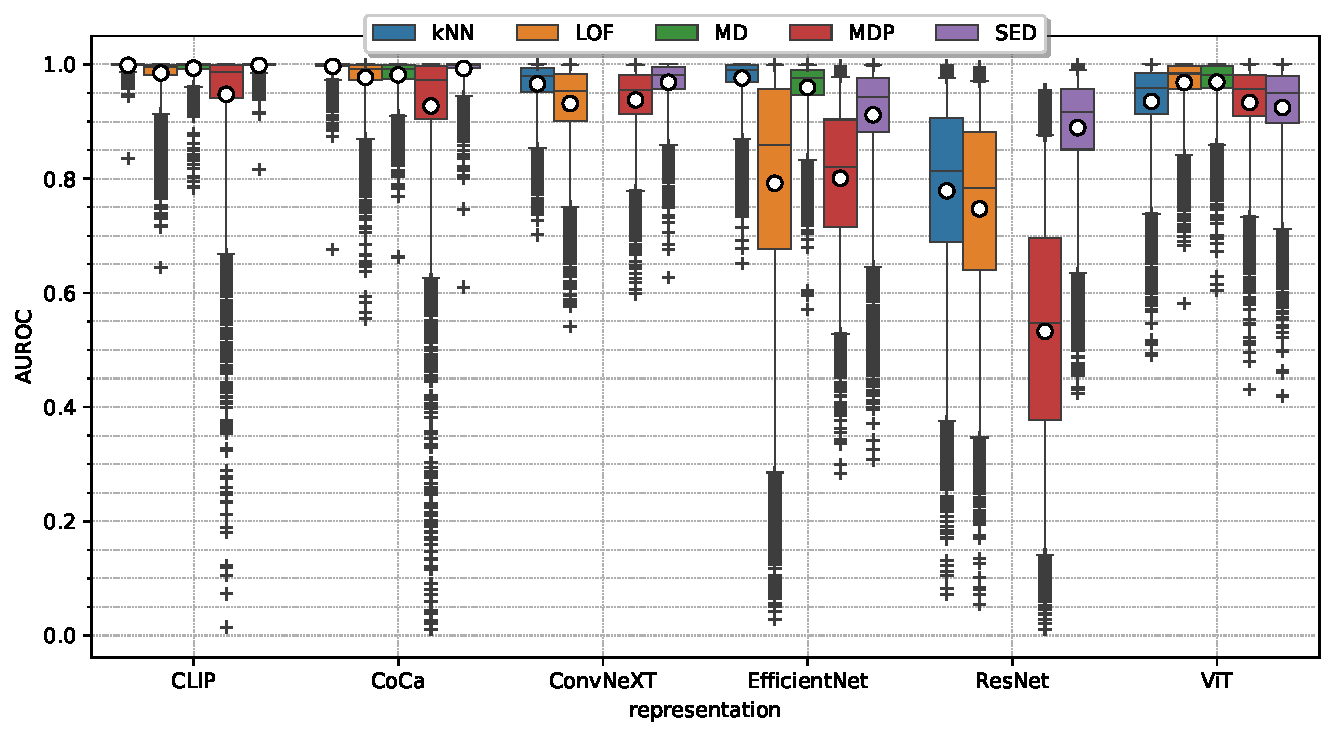
\includegraphics[width=\textwidth]{images/real-separability/barplot-ImageNet-auroc(representation,model)-representation_CLIP,CoCa,ConvNeXT,EfficientNet,ResNet,ViT-class_0,999-data_ALL.pdf}
    \caption{Observed separability between in-distribution data (ImageNet samples) and the out-of-distribution data from 7 datasets: ImageNet-O, iNaturalist, NINCO, OpenImage-O, Places365, SUN2012 and Textures. White dots mark the average scores, while the whiskers indicate the range of 95\% AUROC values calculated for a~given representation and outlierness measure. For some classes (marked with crosses) the~calculated AUROC value is very low, making them indistinguishable from outliers.}
    \label{fig:image-auroc}
    \vspace{-1.0em}  % spacing hack
\end{figure}

\begin{figure}[t]
    % StreamLit settings: width=9, height=4
    \centering
    \vspace{-0.5em}
    \begin{subfigure}[b]{0.9\textwidth}
        \centering
        \caption{\small Separability: ImageNet (ID) vs. ImageNet-O (OOD)}
        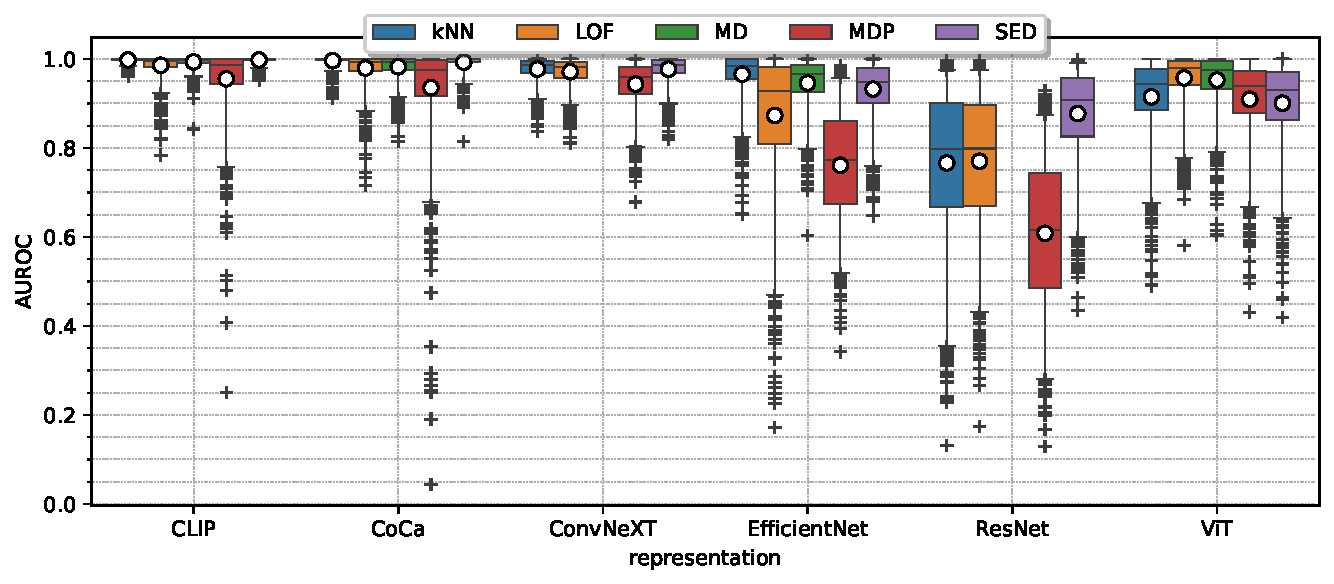
\includegraphics[width=\textwidth]{images/real-separability/barplot-ImageNet-auroc(representation,model)-representation_CLIP,CoCa,ConvNeXT,EfficientNet,ResNet,ViT-class_0,999-data_ImageNet-O.pdf}
        \label{fig:image-auroc-imagenet-o}
    \end{subfigure}

    \vspace{-0.5em}
    \begin{subfigure}[b]{0.9\textwidth}
        \centering
        \caption{\small Separability: ImageNet (ID) vs. Places365 (OOD)}
        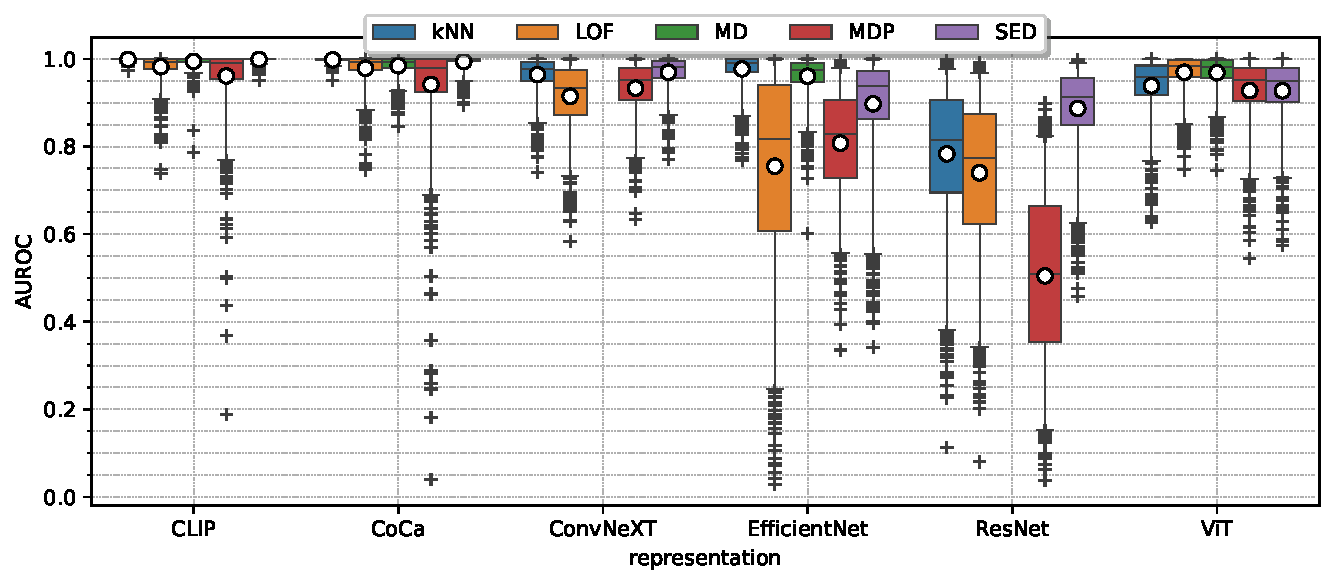
\includegraphics[width=\textwidth]{images/real-separability/barplot-ImageNet-auroc(representation,model)-representation_CLIP,CoCa,ConvNeXT,EfficientNet,ResNet,ViT-class_0,999-data_Places365.pdf}
        \label{fig:image-auroc-places365}
    \end{subfigure}

    \vspace{-0.5em}
    \begin{subfigure}[b]{0.9\textwidth}
        \centering
        \caption{\small Separability: ImageNet (ID) vs. SUN2012 (OOD)}
        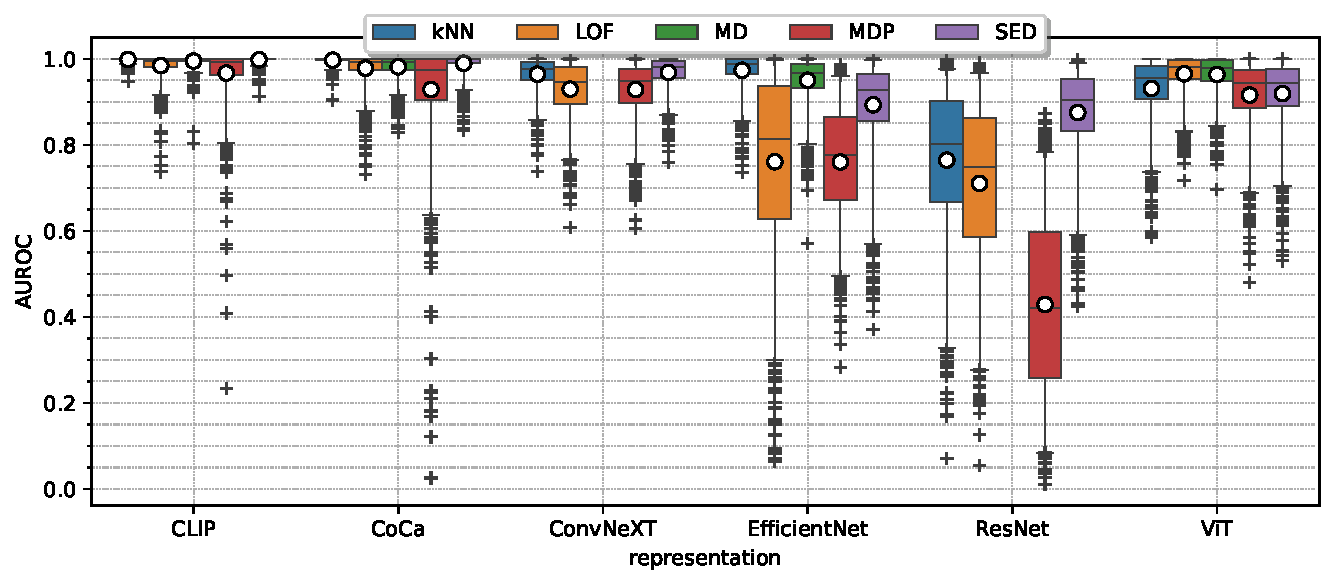
\includegraphics[width=\textwidth]{images/real-separability/barplot-ImageNet-auroc(representation,model)-representation_CLIP,CoCa,ConvNeXT,EfficientNet,ResNet,ViT-class_0,999-data_SUN2012.pdf}
        \label{fig:image-auroc-sun2012}
    \end{subfigure}
    \vspace{-0.5em}
    \caption{Detailed comparison of obtained AUROC scores per selected OOD data. No~major differences can be observed between the analyzed datasets, the utilized representation plays major role along with the chosen outlierness measure.}
    \label{fig:image-auroc-detailed}
\end{figure}

\begin{figure}[t]
    % StreamLit settings: width=9, height=5
    \centering
    \begin{subfigure}[b]{\textwidth}
        \centering
        \caption{\small Separability: 20newsgroups (17 ID classes vs. 3 OOD classes)}
        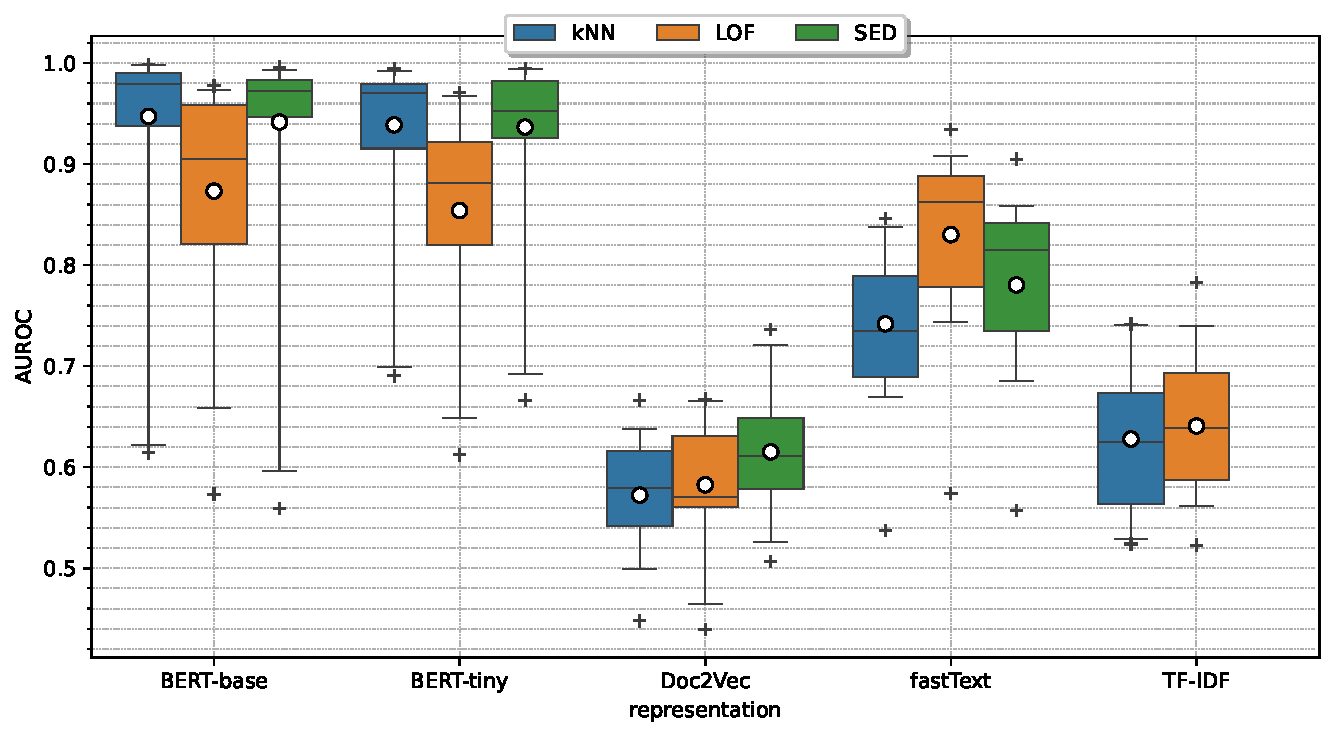
\includegraphics[width=\textwidth]{images/real-separability/barplot-20newsgroups-auroc(representation,model)-representation_BERT-base,BERT-tiny,Doc2Vec,fastText,TF-IDF-class_0,16-data_outlier.pdf}
        \label{fig:text-auroc-20newsgroups}
    \end{subfigure}
    \begin{subfigure}[b]{\textwidth}
        \centering
        \caption{\small Separability: banking77 (62 ID classes vs. 15 OOD classes)}
        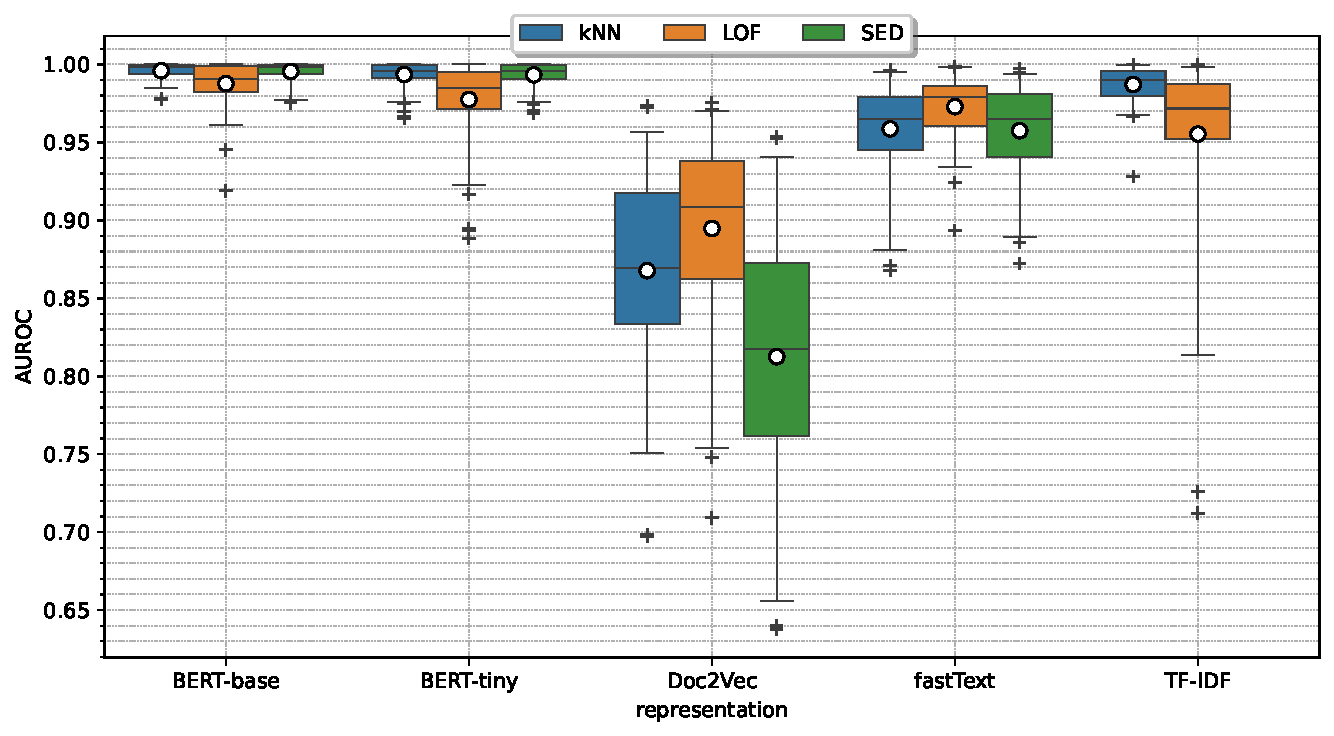
\includegraphics[width=\textwidth]{images/real-separability/barplot-banking77-auroc(representation,model)-representation_BERT-base,BERT-tiny,Doc2Vec,fastText,TF-IDF-class_0,61-data_outlier.pdf}
        \label{fig:text-auroc-banking77}
    \end{subfigure}
    \caption{Calculated AUROC scores, obtained in the separation task between the text data. In case of short documents (banking77) the separation task turns out to be much easier for all analyzed representations (all scores $\text{AUROC} \gtrsim 0.7$). The Doc2Vec and TF-IDF representations for 20newsgroups do not provide vectors suitable for performing the out-of-distribution detection.}
    \label{fig:text-auroc}
\end{figure}

\cleardoublepage{}

\section{Performance of OOD detectors calibrated on training ID data}
\label{section:real-classification}

Figure \ref{fig:image-classification} presents the analysis of recognition capabilities for outlierness measures and utilized representation models. The classification of testing samples was performed with respect to the training data – calibrated so that the 95\% of training samples are properly recognized as in-distribution data. Just like in case of AUROC scores, the~obtained scores for each measure differ between representations and no single universal recommendation can be given.

The results show similar observation as made with the numerical simulations (chapter~\ref{chapter:simulations}) for MD – in considered experiment layout (ImageNet as training data), the available number of training samples $n$ was too low for the dimension $d$ of feature space, so the measure's sensitivity was dramatically low. Under the given criteria, i.e., recognition with respect to the training samples, MD spuriously recognizes all in-distribution testing samples as outliers. However, as per figure \ref{fig:image-auroc}, the MD offers satisfying separability between ID and OOD data (i.e., reaching one of the top AUROC scores), at least in cases where it was possible to utilize (except ConvNeXT and ResNet). This suggest a~potential for MD being a~fine OOD detector, although a~practical utilization in such conditions would requite the threshold calibration using validation data – which is still at least questionable recommendation in the context of robustness and safety-critical applications.

An~alternative commonly proposed in literature for such cases is the utilization of MD variant with pooled covariance matrix – MDP. This variant performs surprisingly well in terms of in-distribution samples recognition (sensitivity), while also maintaining satisfying specificity in most of the cases (except EfficientNet and ResNet). Yet, the best outlierness method overall in this task appears to be SED, reaching top scores for both sensitivity and specificity for every representation except for EfficientNet, where the best measure turned out to be kNN.

The result of classification performed on text documents are presented in figure \ref{fig:text-classification} for completeness. The best metric overall appears to be LOF here, competing closely with SED and kNN for BERT representation. Notably the observed scores are higher for classification task on the short text documents (banking77).

Note the accuracy metric is not presented in this chapter, as due to experiment organization (50 ID samples vs thousands of OOD examples) the results would be heavily biased towards the specificity value anyway. Hence, only the sensitivity and specificity metrics are used for comparison.


\begin{figure}[t]
    % StreamLit settings: width=9, height=5
    \centering
    \begin{subfigure}[b]{\textwidth}
        \centering
        \caption{\small Correctly recognized in-distribution samples (ImageNet)}
        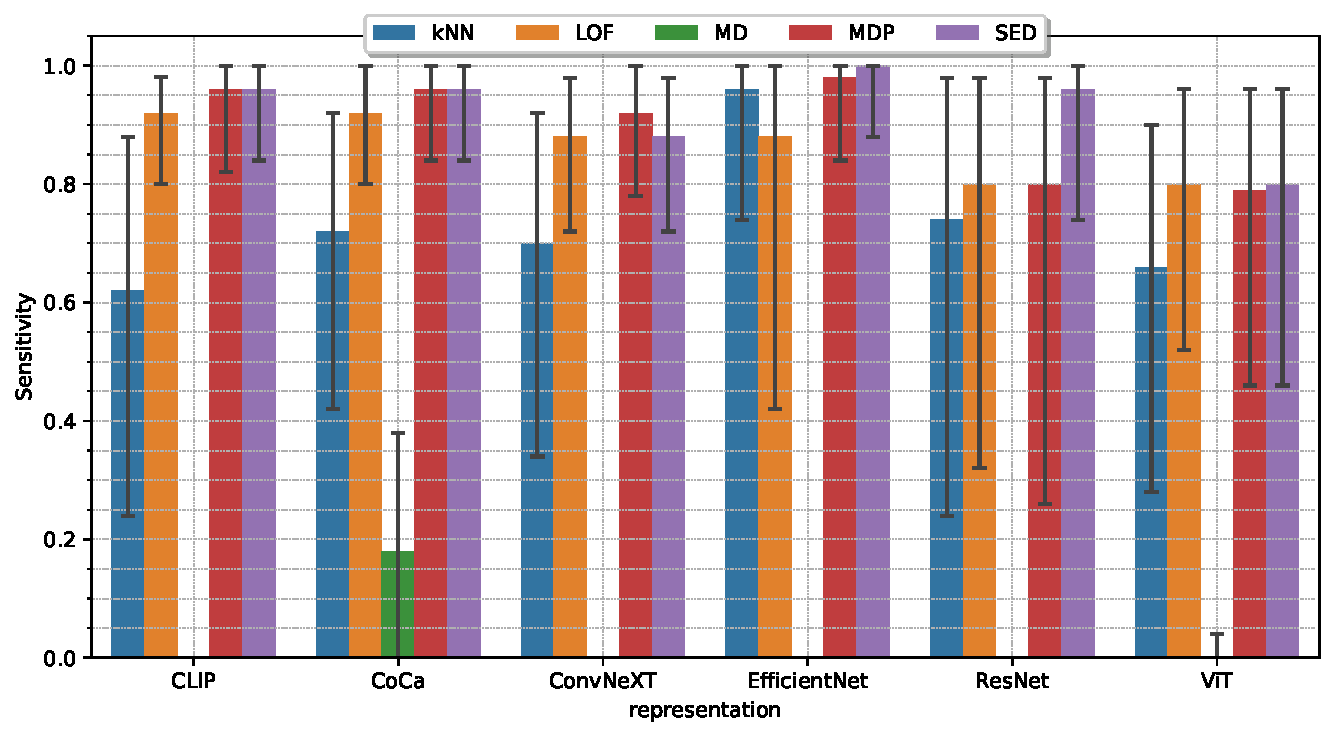
\includegraphics[width=\textwidth]{images/real-classification/barplot-ImageNet-sens_95(representation,model)-representation_CLIP,CoCa,ConvNeXT,EfficientNet,ResNet,ViT-class_0,999-data_ALL.pdf}
        \label{fig:imagenet-sensitivity}
    \end{subfigure}
    \begin{subfigure}[b]{\textwidth}
        \centering
        \caption{\small Correctly recognized out-of-distribution samples (outliers)}
        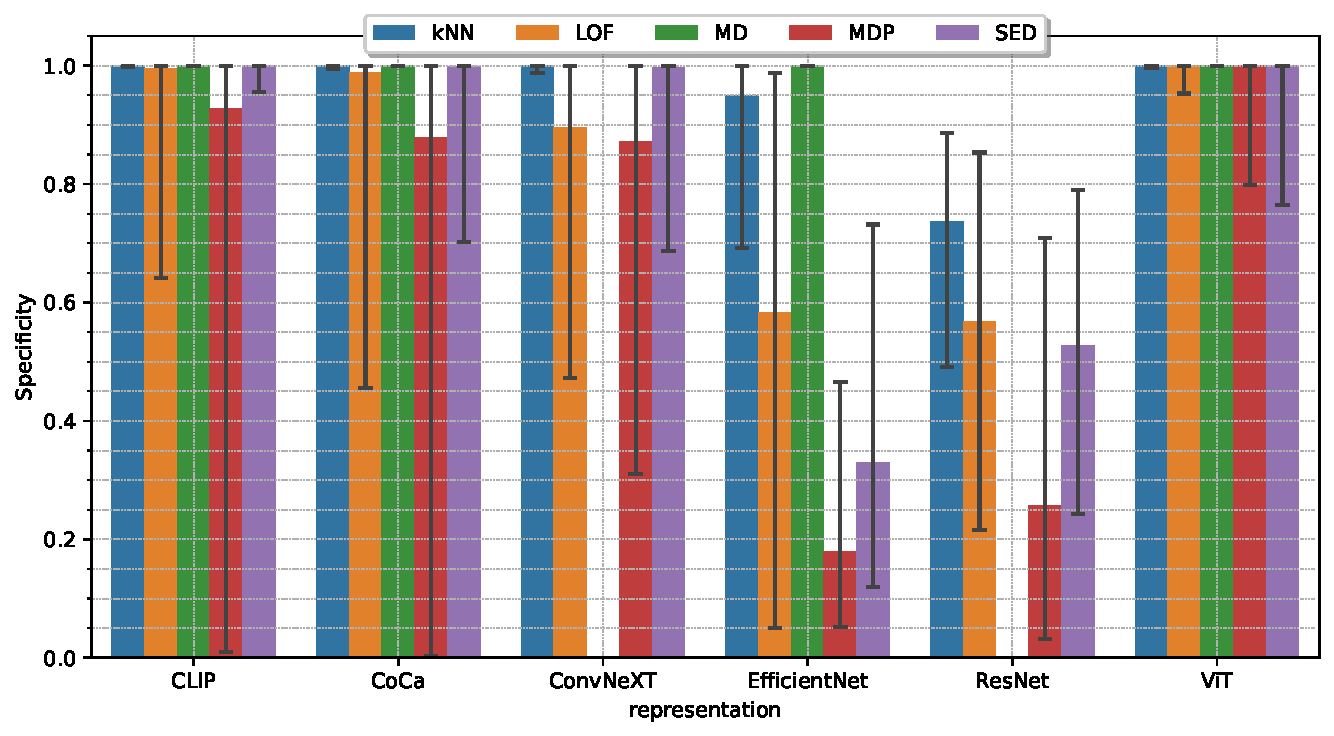
\includegraphics[width=\textwidth]{images/real-classification/barplot-ImageNet-spec_95(representation,model)-representation_CLIP,CoCa,ConvNeXT,EfficientNet,ResNet,ViT-class_0,999-data_ALL.pdf}
        \label{fig:imagenet-specificity}
    \end{subfigure}
    \caption{Results of the image data classification with respect to the training samples. Rejection threshold set so that 95\% of the training data would be correctly recognized as in-distribution. Outliers consist of samples from 7 datasets: ImageNet-O, iNaturalist, NINCO, OpenImage-O, Places365, SUN2012 and Textures.}
    \label{fig:image-classification}
\end{figure}

\begin{figure}[t]
    % StreamLit settings: width=9, height=3
    \centering
    \begin{subfigure}[b]{0.9\textwidth}
        \centering
        \caption{\small Correctly recognized in-distribution samples (20newsgroups)}
        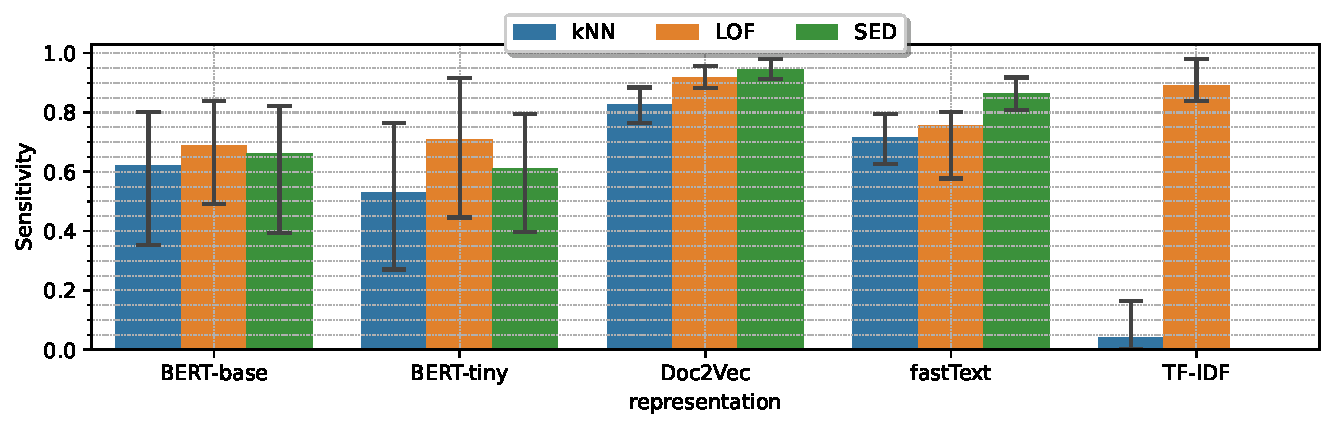
\includegraphics[width=\textwidth]{images/real-classification/barplot-20newsgroups-sens_95(representation,model)-representation_BERT-base,BERT-tiny,Doc2Vec,fastText,TF-IDF-class_0,16-data_outlier.pdf}
        \label{fig:20newsgroups-sensitivity}
    \end{subfigure}

    \vspace{-0.5em}
    \begin{subfigure}[b]{0.9\textwidth}
        \centering
        \caption{\small Correctly recognized out-of-distribution samples (20newsgroups outliers)}
        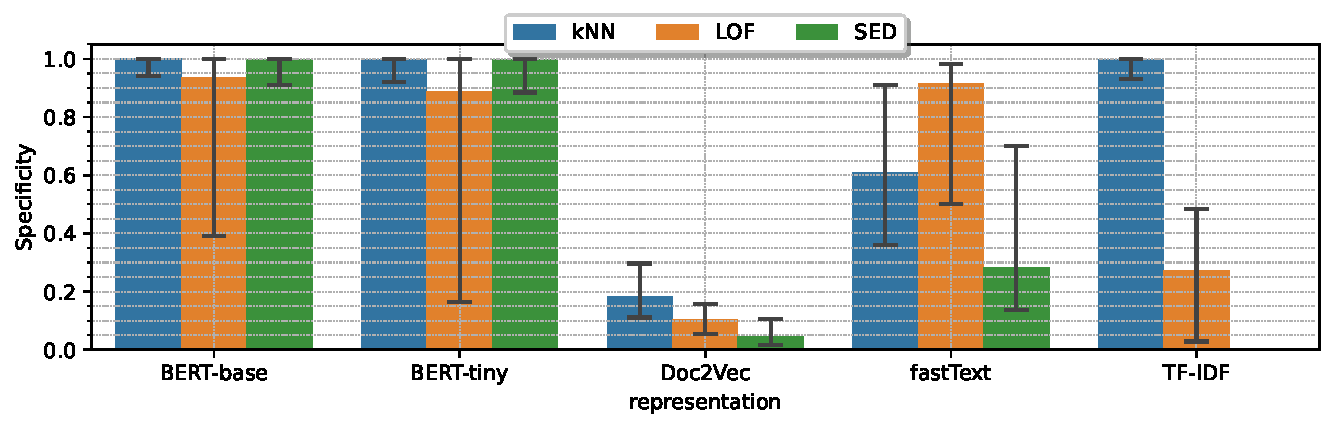
\includegraphics[width=\textwidth]{images/real-classification/barplot-20newsgroups-spec_95(representation,model)-representation_BERT-base,BERT-tiny,Doc2Vec,fastText,TF-IDF-class_0,16-data_outlier.pdf}
        \label{fig:20newsgroups-specificity}
    \end{subfigure}

    \begin{subfigure}[b]{0.9\textwidth}
        \centering
        \caption{\small Correctly recognized in-distribution samples (banking77)}
        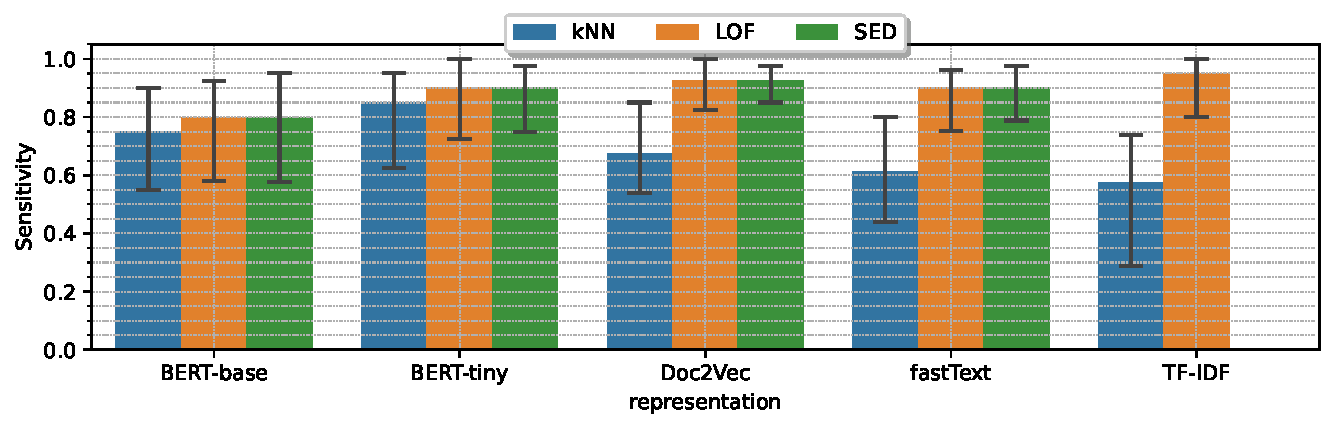
\includegraphics[width=\textwidth]{images/real-classification/barplot-banking77-sens_95(representation,model)-representation_BERT-base,BERT-tiny,Doc2Vec,fastText,TF-IDF-class_0,61-data_outlier.pdf}
        \label{fig:banking77-sensitivity}
    \end{subfigure}

    \vspace{-0.5em}
    \begin{subfigure}[b]{0.9\textwidth}
        \centering
        \caption{\small Correctly recognized out-of-distribution samples (banking77 outliers)}
        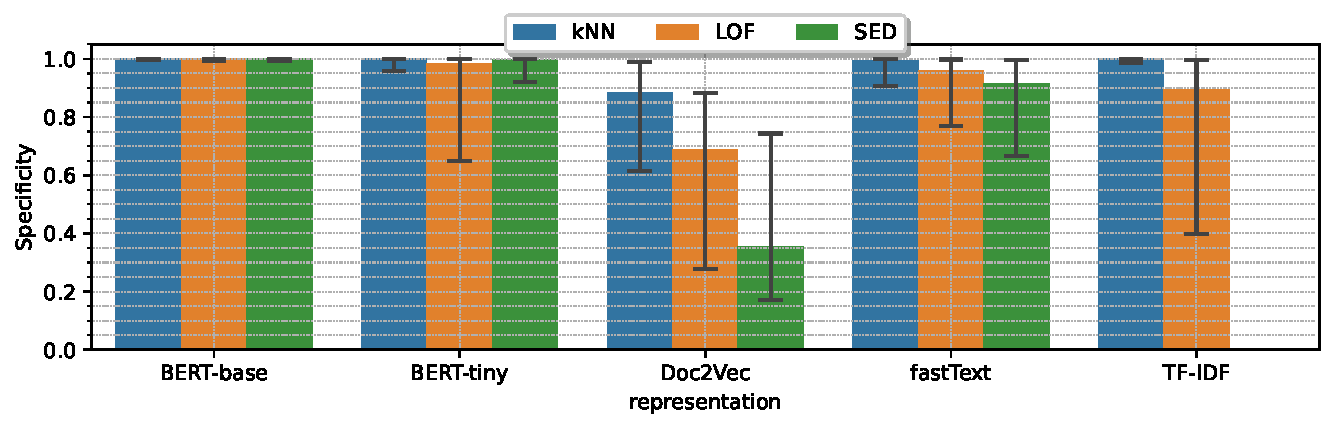
\includegraphics[width=\textwidth]{images/real-classification/barplot-banking77-spec_95(representation,model)-representation_BERT-base,BERT-tiny,Doc2Vec,fastText,TF-IDF-class_0,61-data_outlier.pdf}
        \label{fig:banking77-specificity}
    \end{subfigure}

    \caption{The classification of text documents with respect to the training datasets. Rejection threshold set at $TPR = 95\%$ of the scores obtained for training data.}
    \label{fig:text-classification}
    \vspace{-1.5em}
\end{figure}

\cleardoublepage{}

\section{Characteristics of feature vectors}
\label{section:real-characteristics}

This section contains the analysis and discussion on the properties of the data representations generated by various Deep Learning models –~and how these properties affect (or not) the performance of OOD detection methods. The results correspond to observations made in previous sections (e.g., table \ref{tab:image-auroc}, figures \ref{fig:image-auroc}, \ref{fig:text-auroc}, \ref{fig:image-classification} and \ref{fig:text-classification}).

The table \ref{tab:image-dimensions} summarizes the dimensionality of feature vectors for image data –~coming from the utilized representations models (CLIP, CoCa, ConvNeXT, EfficientNet, ResNet, ViT). The table \ref{tab:text-dimensions} covers analogous information regarding the feature vectors obtained for text documents from models (BERT, Doc2Vec, fastText, TF-IDF).

Figures \ref{fig:characteristics-image}, \ref{fig:characteristics-text-20newsgroups}, \ref{fig:characteristics-text-banking77} illustrate the various discovered properties of the feature vectors, per in-distribution data class and utilized representation model, obtained for the image data (ImageNet), long (20newsgroups) and short (banking77) text documents, respectively. The considered values are as follows:
\vspace{-0.5\baselineskip}
\begin{itemize}
    \item variance – calculated as an average value over all features in a given class,
    \item correlation – an average of the absolute values calculated within the top triangle of the covariance matrix,
    \item kurtosis – computed as an average over all features for each class; value $3.0$ corresponds to normal-like distribution, big values indicate long tails, low values are related to highly-concentrated data.
    \item skewness – also calculated as an average value over all features; values in range $(-0.5, 0.5)$ mean that distribution is approximately symmetric, for values $(0.5, 1.0)$ the distribution is slightly skewed and for values $(1.0; \infty)$ it is considered a~highly skewed distribution.
    \item test of normality – average $p$-value obtained for each feature in class, using the D’Agostino and Pearson’s test\footnote{\url{https://docs.scipy.org/doc/scipy/reference/generated/scipy.stats.normaltest.html}} with assumption of the Gaussian distribution as~the~null-hypothesis.
    \item number of feature-wise outliers – the average number of observations that fall outside the confidence interval (range $\pm1.5$ IQR threshold) based on the values of each feature in the training clusters vectors.
\end{itemize}

Important observation for all the analyzed cases is that, in general, there are no strongly correlated features – all medians of absolute correlations are below $0.25$. However the observed correlations vary per class, especially significantly for some representations (EfficientNet and BERT), and this raises the question of justification for utilization of the pooled covariance matrix. As classes present various correlations, the single covariance matrix incorrectly reflects data from some of these classes, i.e., it~results in an~important method error, visible as low performance of MDP measure.

The features produced by ResNet are especially weakly correlated, which corresponds with high efficiency of SED measure with this representation in conducted experiments. Contrary, EfficientNet is characterized by higher correlations, hence the MD performs better than SED in that case (i.e., ignoring the correlations leads to worse performance).

Similarly, there are no significant differences in average variances of features observed. Although the BERT, CoCa and fastText produced feature vectors of especially low average variance. Most representations produce features that appear symmetric (BERT, CLIP, CoCa, ConvNeXT, Doc2Vec, fastText and ViT), with exception of EfficientNet and ResNet, where the valued are highly skewed – and additionally, in case of ResNet, widely distributed with long tails.

For TF-IDF the SED measure was impossible to utilize due to multiple empty features in obtained vectors, i.e., zero-variance calculated and therefore division by zero encountered in formula \ref{eq:sed} (section \ref{section:SEuclidean}). Also, because of the TF-IDF feature vectors sizes, the estimation of properties such as correlations was time-consuming and hence it is omitted in the figures.

It must be noticed that the characteristics obtained for short and long text documents differ significantly in some cases, e.g., in the normality tests (figures \ref{fig:text-20newsgroups-pvalue} and \ref{fig:text-banking77-pvalue}). This corresponds with inconsistencies observed fpr results of AUROC, sensitivity and specificity scores between 20newsgroups and banking77, presented in previous sections. Hence, a more detailed study of the relation between the characteristics and the ID data shall be conducted in the future.

\begin{table}[t]
    \centering
    \small
    \setlength{\tabcolsep}{0.56em}
    \renewcommand{\arraystretch}{1.5}
    \begin{tabular}{l|ccccccc}
        \toprule
        \toprule
            representation
            & CLIP
            & CoCa
            & ConvNeXT
            & EfficientNet
            & MobileNet
            & ResNet
            & ViT
            \\
        \midrule
            dimension $d$
            & 1024
            & 769
            & 1536
            & 1280
            & 1280
            & 2048
            & 1024
            \\
        \bottomrule
        \bottomrule
    \end{tabular}
    \caption{Dimensionality of the feature vectors used for image representations.}
    \label{tab:image-dimensions}
    \vspace{-0.5em}  % spacing hack
    \begin{tabular}{l|cccccc}
        \toprule
        \toprule
            representation
            & BERT-base
            & BERT-tiny
            & Doc2Vec
            & fastText
            & ${}^\text{~~~~TF-IDF}_\text{\tiny(20newsgroups)}$
            & ${}^\text{~\,TF-IDF}_\text{\tiny(banking77)}$
            \\
        \midrule
            dimension $d$
            & 768
            & 128
            & 300
            & 100
            & 5000
            & 2095
            \\
        \bottomrule
        \bottomrule
    \end{tabular}
    \caption{Dimensionality of the feature vectors used for text representations.}
    \label{tab:text-dimensions}
    \vspace{-1.8em}  % spacing hack
\end{table}

\begin{figure}[t]
    % StreamLit settings: width=5, height=3
    \centering
    \begin{subfigure}[b]{0.495\textwidth}
        \centering
        \caption{\small Correlation of features}
        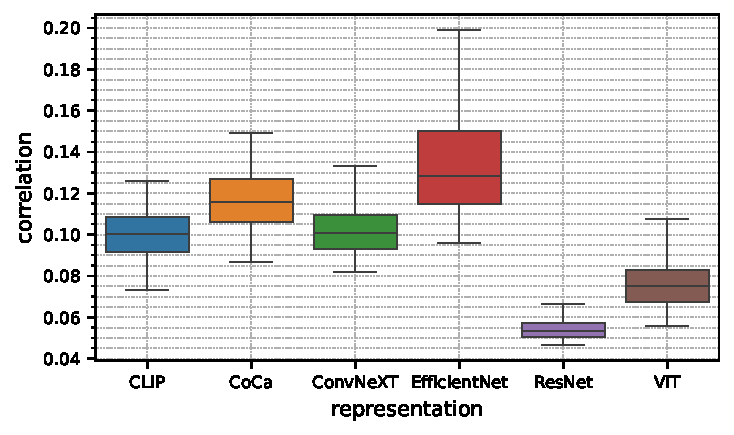
\includegraphics[width=\textwidth]{images/real-characteristics/image/properties-ImageNet-abscorr(representation,representation)-representation_CLIP,CoCa,ConvNeXT,EfficientNet,ResNet,ViT-class_0,999-data_ID-train.pdf}
        \label{fig:image-abscorr}
    \end{subfigure}
    \hfill
    \begin{subfigure}[b]{0.495\textwidth}
        \centering
        \caption{\small Variance of features}
        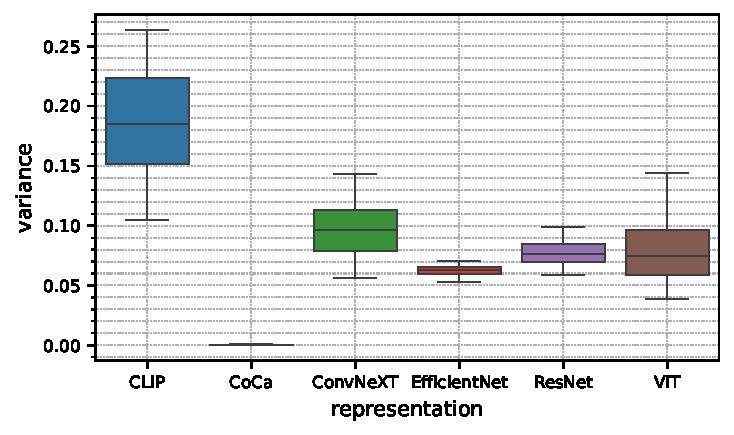
\includegraphics[width=\textwidth]{images/real-characteristics/image/properties-ImageNet-var(representation,representation)-representation_CLIP,CoCa,ConvNeXT,EfficientNet,ResNet,ViT-class_0,999-data_ID-train.pdf}
        \label{fig:image-var}
    \end{subfigure}
    \begin{subfigure}[b]{0.495\textwidth}
        \centering
        \caption{\small Number of outliers per feature}
        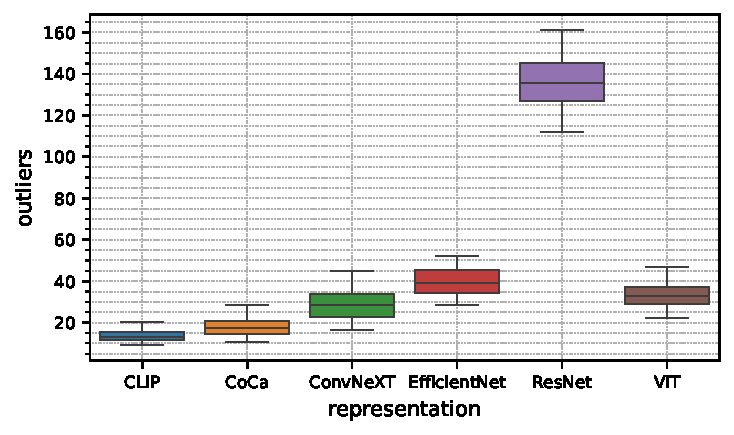
\includegraphics[width=\textwidth]{images/real-characteristics/image/properties-ImageNet-noutliers(representation,representation)-representation_CLIP,CoCa,ConvNeXT,EfficientNet,ResNet,ViT-class_0,999-data_ID-train.pdf}
        \label{fig:image-outliers}
    \end{subfigure}
    \hfill
    \begin{subfigure}[b]{0.495\textwidth}
        \centering
        \caption{\small Test of features normality}
        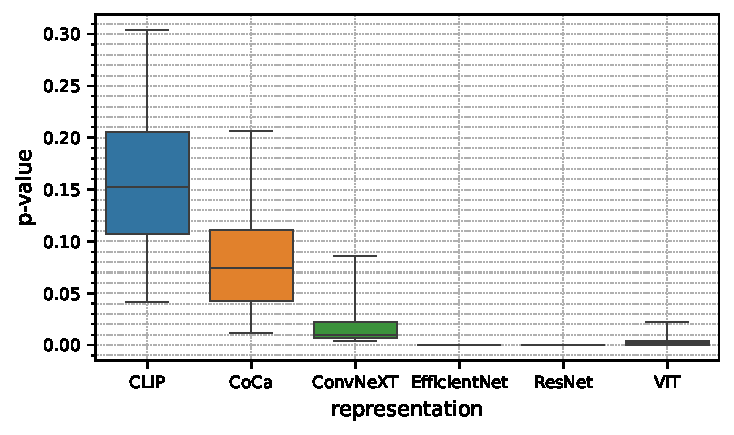
\includegraphics[width=\textwidth]{images/real-characteristics/image/properties-ImageNet-pval(representation,representation)-representation_CLIP,CoCa,ConvNeXT,EfficientNet,ResNet,ViT-class_0,999-data_ID-train.pdf}
        \label{fig:image-pvalue}
    \end{subfigure}
    \begin{subfigure}[b]{0.495\textwidth}
        \centering
        \caption{\small Kurtosis of features}
        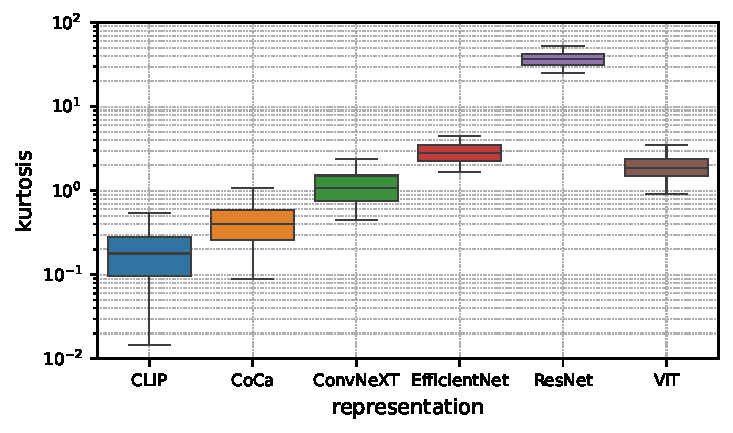
\includegraphics[width=\textwidth]{images/real-characteristics/image/properties-ImageNet-kurt(representation,representation)-representation_CLIP,CoCa,ConvNeXT,EfficientNet,ResNet,ViT-class_0,999-data_ID-train.pdf}
        \label{fig:image-curtosis}
    \end{subfigure}
    \hfill
    \begin{subfigure}[b]{0.495\textwidth}
        \centering
        \caption{\small Skewness of features}
        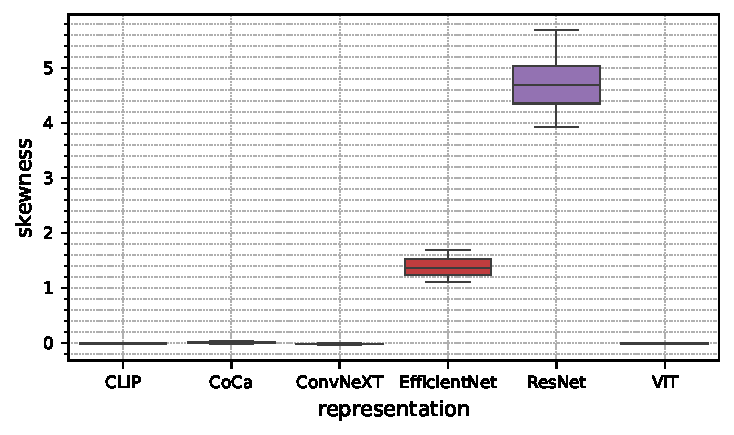
\includegraphics[width=\textwidth]{images/real-characteristics/image/properties-ImageNet-skew(representation,representation)-representation_CLIP,CoCa,ConvNeXT,EfficientNet,ResNet,ViT-class_0,999-data_ID-train.pdf}
        \label{fig:image-skewness}
    \end{subfigure}
    \caption{Properties of feature vectors corresponding to ImageNet classes obtained for 6~different representations algorithms (CLIP, CoCa, ConvNeXT, EfficientNet, ResNet~and~ViT). The same image data can be expressed as a~completely different feature~vector, depending on the chosen representation.}
    \label{fig:characteristics-image}
\end{figure}

\begin{figure}[t]
    % StreamLit settings: width=5, height=3
    \centering
    \begin{subfigure}[b]{0.495\textwidth}
        \centering
        \caption{\small Correlation of features}
        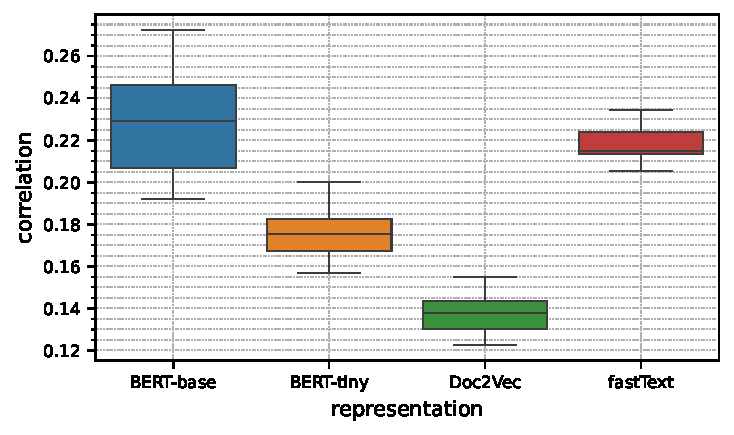
\includegraphics[width=\textwidth]{images/real-characteristics/text-20newsgroups/properties-20newsgroups-abscorr(representation,representation)-representation_BERT-base,BERT-tiny,Doc2Vec,fastText-class_0,16-data_ID-train.pdf}
        \label{fig:text-20newsgroups-abscorr}
    \end{subfigure}
    \hfill
    \begin{subfigure}[b]{0.495\textwidth}
        \centering
        \caption{\small Variance of features}
        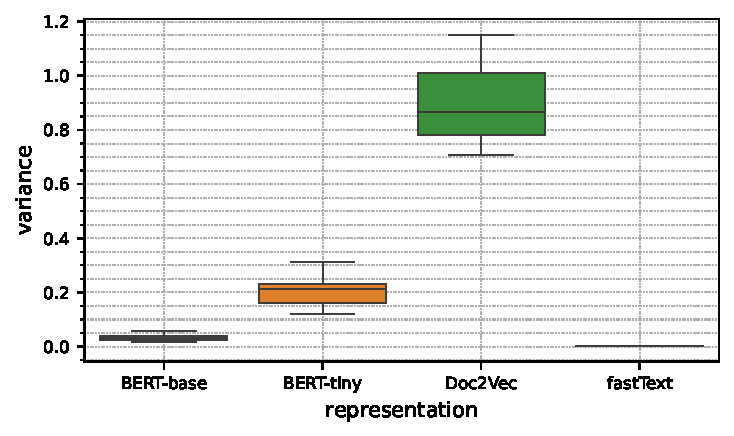
\includegraphics[width=\textwidth]{images/real-characteristics/text-20newsgroups/properties-20newsgroups-var(representation,representation)-representation_BERT-base,BERT-tiny,Doc2Vec,fastText-class_0,16-data_ID-train.pdf}
        \label{fig:text-20newsgroups-var}
    \end{subfigure}
    \begin{subfigure}[b]{0.495\textwidth}
        \centering
        \caption{\small Number of outliers per feature}
        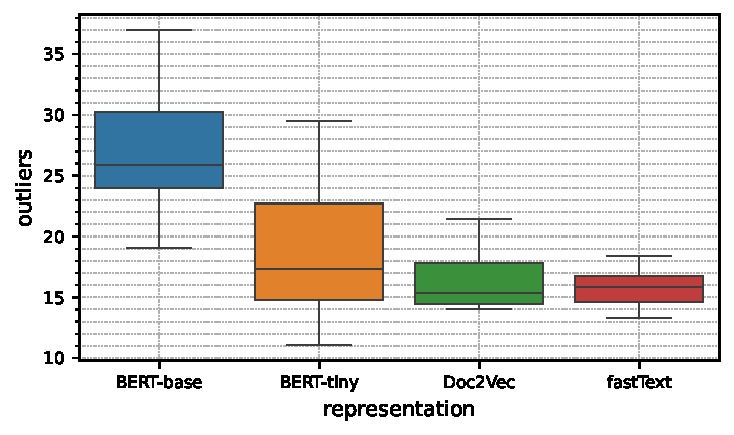
\includegraphics[width=\textwidth]{images/real-characteristics/text-20newsgroups/properties-20newsgroups-noutliers(representation,representation)-representation_BERT-base,BERT-tiny,Doc2Vec,fastText-class_0,16-data_ID-train.pdf}
        \label{fig:text-20newsgroups-outliers}
    \end{subfigure}
    \hfill
    \begin{subfigure}[b]{0.495\textwidth}
        \centering
        \caption{\small Test of features normality}
        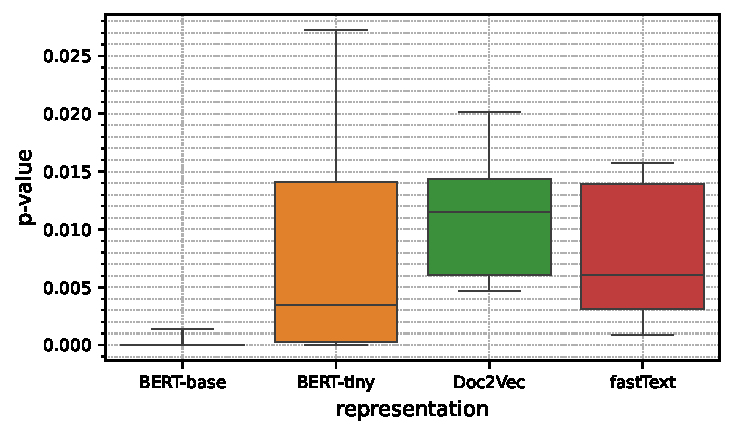
\includegraphics[width=\textwidth]{images/real-characteristics/text-20newsgroups/properties-20newsgroups-pval(representation,representation)-representation_BERT-base,BERT-tiny,Doc2Vec,fastText-class_0,16-data_ID-train.pdf}
        \label{fig:text-20newsgroups-pvalue}
    \end{subfigure}
    \begin{subfigure}[b]{0.495\textwidth}
        \centering
        \caption{\small Kurtosis of features}
        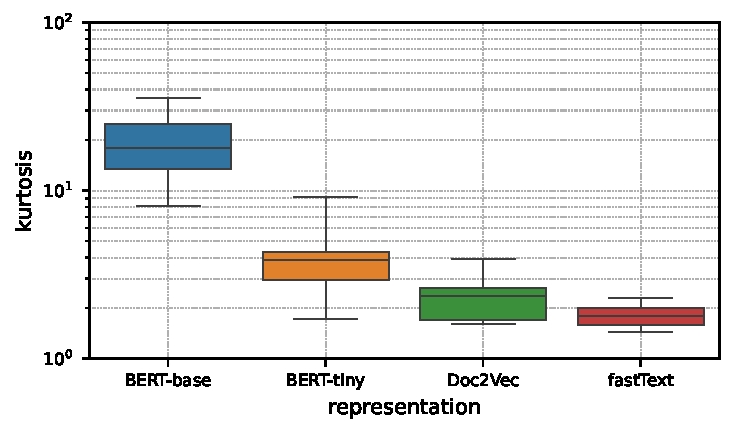
\includegraphics[width=\textwidth]{images/real-characteristics/text-20newsgroups/properties-20newsgroups-kurt(representation,representation)-representation_BERT-base,BERT-tiny,Doc2Vec,fastText-class_0,16-data_ID-train.pdf}
        \label{fig:text-20newsgroups-curtosis}
    \end{subfigure}
    \hfill
    \begin{subfigure}[b]{0.495\textwidth}
        \centering
        \caption{\small Skewness of features}
        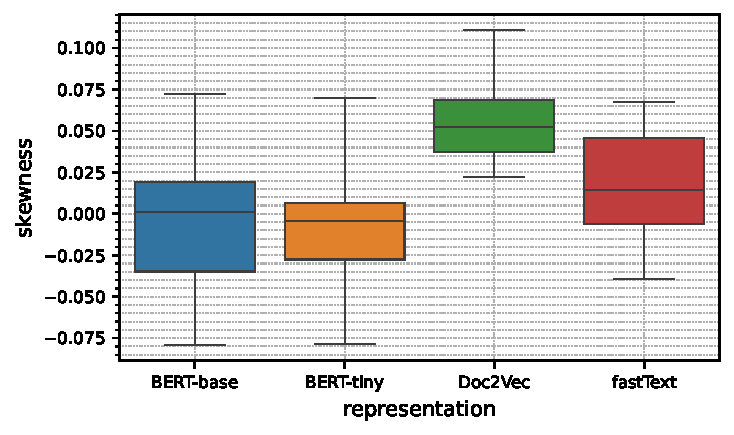
\includegraphics[width=\textwidth]{images/real-characteristics/text-20newsgroups/properties-20newsgroups-skew(representation,representation)-representation_BERT-base,BERT-tiny,Doc2Vec,fastText-class_0,16-data_ID-train.pdf}
        \label{fig:text-20newsgroups-skewness}
    \end{subfigure}
    \caption{Properties of feature vectors corresponding to 20newsgroups classes obtained for different representations algorithms (BERT, Doc2Vec and fastText). Analysis for TF-IDF was omitted due to the size of feature vectors.}
    \label{fig:characteristics-text-20newsgroups}
\end{figure}

\begin{figure}[t]
    % StreamLit settings: width=5, height=3
    \centering
    \begin{subfigure}[b]{0.495\textwidth}
        \centering
        \caption{\small Correlation of features}
        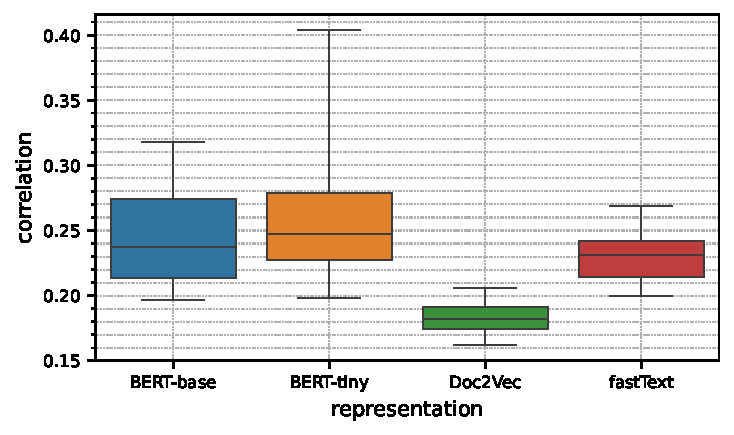
\includegraphics[width=\textwidth]{images/real-characteristics/text-banking77/properties-banking77-abscorr(representation,representation)-representation_BERT-base,BERT-tiny,Doc2Vec,fastText-class_0,61-data_ID-train.pdf}
        \label{fig:text-banking77-abscorr}
    \end{subfigure}
    \hfill
    \begin{subfigure}[b]{0.495\textwidth}
        \centering
        \caption{\small Variance of features}
        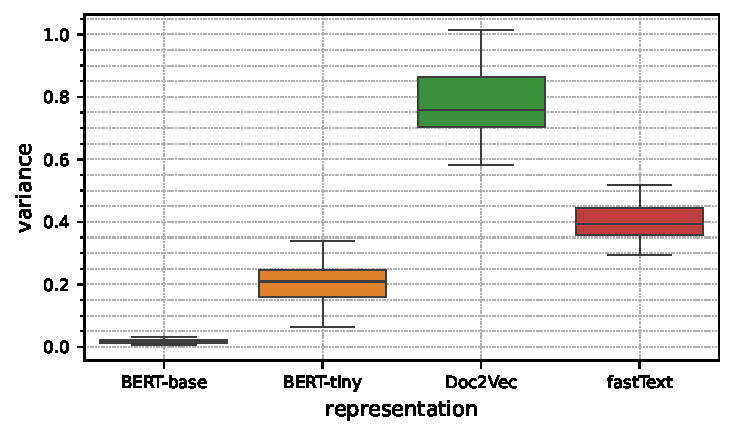
\includegraphics[width=\textwidth]{images/real-characteristics/text-banking77/properties-banking77-var(representation,representation)-representation_BERT-base,BERT-tiny,Doc2Vec,fastText-class_0,61-data_ID-train.pdf}
        \label{fig:text-banking77-var}
    \end{subfigure}
    \begin{subfigure}[b]{0.495\textwidth}
        \centering
        \caption{\small Number of outliers per feature}
        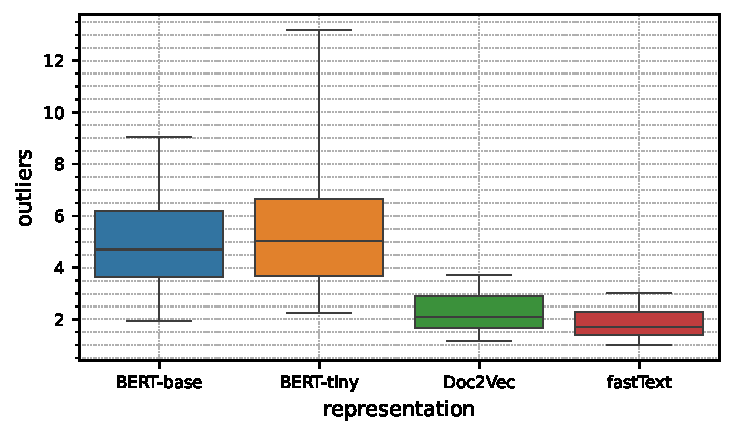
\includegraphics[width=\textwidth]{images/real-characteristics/text-banking77/properties-banking77-noutliers(representation,representation)-representation_BERT-base,BERT-tiny,Doc2Vec,fastText-class_0,61-data_ID-train.pdf}
        \label{fig:text-banking77-outliers}
    \end{subfigure}
    \hfill
    \begin{subfigure}[b]{0.495\textwidth}
        \centering
        \caption{\small Test of features normality}
        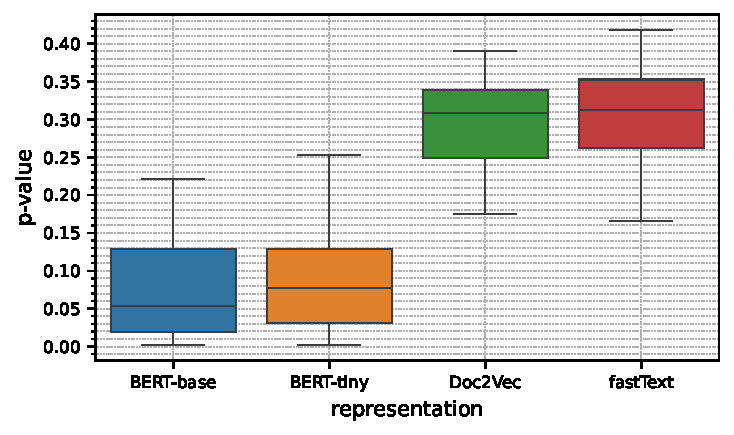
\includegraphics[width=\textwidth]{images/real-characteristics/text-banking77/properties-banking77-pval(representation,representation)-representation_BERT-base,BERT-tiny,Doc2Vec,fastText-class_0,61-data_ID-train.pdf}
        \label{fig:text-banking77-pvalue}
    \end{subfigure}
    \begin{subfigure}[b]{0.495\textwidth}
        \centering
        \caption{\small Kurtosis of features}
        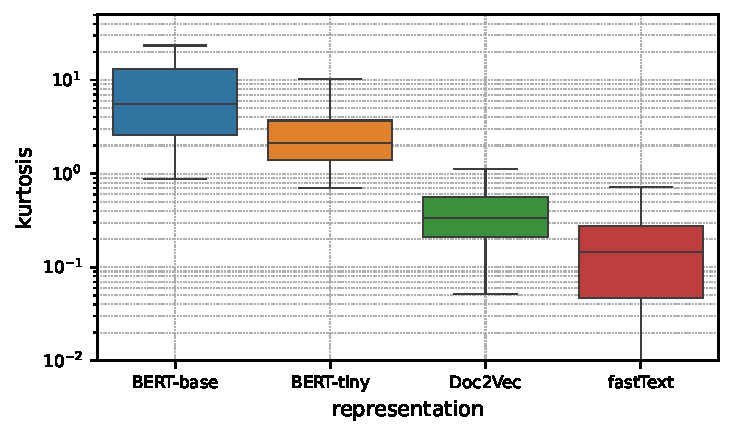
\includegraphics[width=\textwidth]{images/real-characteristics/text-banking77/properties-banking77-kurt(representation,representation)-representation_BERT-base,BERT-tiny,Doc2Vec,fastText-class_0,61-data_ID-train.pdf}
        \label{fig:text-banking77-curtosis}
    \end{subfigure}
    \hfill
    \begin{subfigure}[b]{0.495\textwidth}
        \centering
        \caption{\small Skewness of features}
        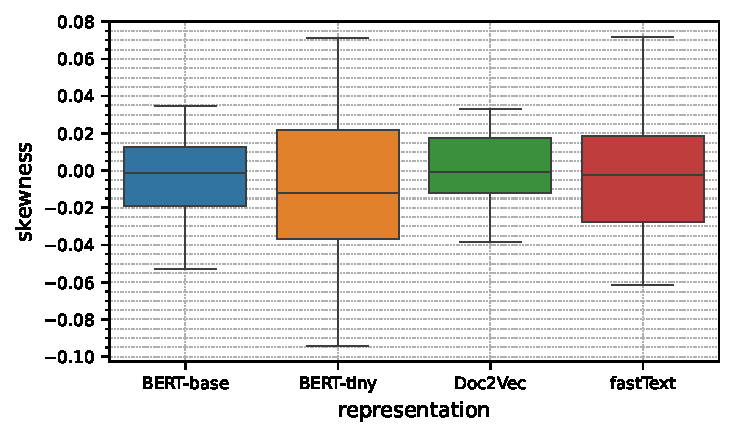
\includegraphics[width=\textwidth]{images/real-characteristics/text-banking77/properties-banking77-skew(representation,representation)-representation_BERT-base,BERT-tiny,Doc2Vec,fastText-class_0,61-data_ID-train.pdf}
        \label{fig:text-banking77-skewness}
    \end{subfigure}
    \caption{Properties of feature vectors corresponding to banking77 classes obtained for different representations algorithms (BERT, Doc2Vec and fastText). Analysis~for~TF-IDF was omitted due to the size of feature vectors.}
    \label{fig:characteristics-text-banking77}
\end{figure}

\cleardoublepage{}


    \cleardoublepage

    \chapter{Summary}
\label{chapter:summary}

In this work the problem of open-set classification in high-dimensional feature spaces was explored. It is a~key task to be solved to ensure the security of implementations and the reliability of machine learning models – in particular: deep learning models for image and text recognition; allowing the systems that utilize such models to react predictably to new data and unexpected situations. Although the~problem remains open, the conducted research contributes to the field, introducing new insights of the selected \textit{post-hoc} methods behaviors and properties, as well as providing recommendations of outlierness measures and high-dimensional representation techniques for applications involving image and text data.

A comprehensive study on the performance of selected \textit{post-hoc} methods for outliers detection was conducted. Primarily, it was shown that the performance of OOD detectors is dependent on the properties of the representation – i.e., of the feature space in which the recognition of outliers is performed. This problem is not sufficiently noticed in the existing literature – the rankings of methods in benchmarks are presented, comparing results for various representations or showing results for a~fixed selected representation (usually ResNet) without emphasizing it, making the formulated general conclusions turning out to be not useful when new representations or out-of-distribution detection methods are analyzed.

One of the most interesting observation is related to the phenomenon that the measures can consider training and testing data coming from the same distribution (ID) as distant from each other, i.e., testing data may be considered outliers with respect to the available training samples. For ED, SED and IRWD measures it is only observed for highly under-represented training cluster for a~given dimension, i.e., $n \ll d$, and quickly vanishes as number of training samples grows. For MD measure this phenomenon is observed unless a~significantly great number of training samples is provided, $n \gg d$, which in high-dimensional feature spaces becomes troublesome. In case of kNN, the phenomenon is also observed and it is related to the selected value of $k$ – for low value $k$ the train-test distance is greater than for higher values of $k$. Detailed research of this effect for kNN shall be conducted in the future. For ABOF and LOF measures this phenomenon was not observed even under extreme conditions.

Despite the observed train-test data distancing, all analyzed outlierness measures can still reliably distinct the in-distribution (ID) data from sufficiently distant out-of-distribution (OOD, outliers), which is proven by the calculated AUROC scores. However, this means that in some cases, notably for MD and kNN, the threshold calibration for the open-set classification task requires involvement of the additional validation in-distribution data to achieve correct results, although reliability of such approach may be questionable.

For all analyzed measures, the more distant the outliers were from the in-distribution samples, the higher AUROC scores were observed. Contrary, higher dimension $d$ of feature vectors made the separability between in-distribution and out-of-distributon data more challenging. The number of training samples $n$ did not affect much the methods performance for a~given fixed $d$ and~$h$, except for the extreme conditions (e.g.~$n < 10^2$ for $d = 750$) or MD measure, where there is a~computational requirement $n \geq d$ (condition for inverting the covariance matrix used in distance formula).

The results of numerical study were compared with the open-set classification task conduced on the real-world data, utilizing feature vectors produced by multiple representation algorithms – CLIP, CoCa, ConvNeXT, EfficientNet, ResNet and Vit for image data; BERT, Doc2Vec, fastText and TF-IDF for text documents. Future work in this field shall conduct more comprehensive study, involving the research focused on other domains than image and text recognition – for example AI in medicine, such as the bacteria identification based on genomic sequences \cite{Ren-2019}\cite{Fort-2021}, where the OOD detection is the essential element in real-world applications.

It was shown that for all analyzed cases there exist a~notable number of classes that contain samples much more difficult to distinguish from outliers. Such classes pose an~important security gap in the deployed machine learning system. Hence, the per-class analysis of~ID-OOD separability is proposed as a~recommended approach any safety-critical applications.
Further work in this topic should involve a~detailed focus on those classes – the curious question remains if those are the same classes for all outlierness measures and representation algorithms, and notably why such classes are characterized by poor performance in the outliers detection task.


\section{Recommendations for OOD detection with Deep Learning models}
\label{section:real-recommendations}

Based on the conducted study, the following recommendations regarding the usage of OOD detection methods can be formulated, assuming the task in image and text recognition domain using Deep Learning representation methods.
\vspace{-0.5\baselineskip}
\begin{enumerate}
    \item The OOD detector based on the Mahalanobis distance with a single, common covariance matrix for all classes of the known ID set (i.e., pooled variant, MDP) should be avoided and not used – it is always less effective in outlier detection task than the original variant (MD), which involves a separate covariance matrix calculated for each ID class, or the variant with diagonal covariance matrix (SED), which assumes no correlations between features. The selection between MD and SED can be made by analysis of the representation characteristics – for model with no or low correlations of features, such as ResNet, the SED is preferred.
    \item The operating point, i.e., OOD detection threshold (formula \ref{eq:open-set-classification}), of detectors based on popular kNN and MD measures, cannot be calibrated on the condition that a~given fraction of training data (e.g., $95\%$) will be correctly recognized. For~such measures, the procedure results in a~low sensitivity of ID recognition by the detector. An additional, independent set of validation data must be used to calibrate detectors based on such measures. However, other OOD detectors, e.g., utilizing LOF and SED, can be successfully calibrated on just the training in-distribution (ID) data.
    \item The selection of OOD detector in real-world implementations of the Machine Learning systems should be made based on the analysis of the representations characteristics generated by the Deep Learning models. For example, for the ResNet model the preferred OOD detector involves SED measure, while for the ViT model both LOF and MD performs best. The OOD detector rankings and recommendations made for a fixed representation (Deep Learning model) do not transfer to other models.
    \item The data representation models generated by various Deep Learning techniques (e.g., CNN, ViT, CLIP) differ significantly in therms of OOD-generalization, i.e., the~susceptibility to errors of incorrect identifications of OOD observations. Hence, in any safety-critical task, it is recommended to utilize either CLIP, CoCa or ConvNeXT models, as offering the best results in general. Models such as ResNet, EfficientNet and ViT bear a~greater risk of OOD data incorrect recognition.
    \item The implementation of the AI system in the real-world tasks, especially for safety-critical ones, should be preceded with an analysis of OOD-generalization per every known class. This will allow to identify the security gaps in the system by capturing the classes with low OOD-generalization, i.e., classes that are easier to confuse with out-of-distribution data, i.e., are more prone to incorrect recognition.
\end{enumerate}

Relying on these above recommendations will improve the quality of OOD observations recognition, therefore resulting in improved trustworthiness of Machine Learning systems in real-world and safety-critical applications.

\cleardoublepage{}

    \cleardoublepage


    \appendix

    \chapter{Glossary}
\label{chapter:glossary}

\todo{Do zrobienia}  % TODO
\lipsum[1]

    \cleardoublepage

    \chapter{Source code}
\label{chapter:source-code}

\todo{Do zrobienia}  % TODO
\lipsum[1]

    \cleardoublepage

    \chapter{Selected personal achievements}
\label{chapter:achievements}

This chapter covers the author's personal background.


\section{List of scientific publications}
\label{section:publications}

Detailed list can be found in the database of the Wrocław University of Science and~Technology: \url{https://dona.pwr.edu.pl/szukaj/default.aspx?nrewid=600305}

\begin{itemize}
    \item
        \underline{Szymon Datko}, Henryk Maciejewski, Tomasz Walkowiak,
        \textit{“Measures of Outlierness in High-Dimensional Data under Correlation of Features - with Application for Open-Set Classification“},
        proceedings of the Seventeenth International Conference on Dependability of Computer Systems, DepCoS-RELCOMEX, 2022.\\
        \textbf{DOI}: \url{https://doi.org/10.1007/978-3-031-06746-4_3}

    \item
        Tomasz Walkowiak, \underline{Szymon Datko}, Henryk Maciejewski,
        \textit{“Utilizing Local Outlier Factor for Open-Set Classification in High-Dimensional Data - Case Study Applied for Text Documents“},
        Intelligent Systems and Applications: proceedings of the 2019 Intelligent Systems Conference, IntelliSys, 2019.\\
        \textbf{DOI}: \url{https://doi.org/10.1007/978-3-030-29516-5_33}

    \item
        Tomasz Walkowiak, \underline{Szymon Datko}, Henryk Maciejewski,
        \textit{“Distance metrics in Open-Set Classification of Text Documents by Local Outlier Factor and Doc2Vec“},
        Advances and trends in artificial intelligence: from theory to practice: 32nd International Conference on Industrial, Engineering and Other Applications of Applied Intelligent Systems, IEA/AIE, 2019.\\
        \textbf{DOI}: \url{https://doi.org/10.1007/978-3-030-22999-3_10}

    \item
        Tomasz Walkowiak, \underline{Szymon Datko}, Henryk Maciejewski,
        \textit{“Low-dimensional classification of text documents“},
        Engineering in dependability of computer systems and networks: proceedings of the Fourteenth International Conference on Dependability of Computer Systems, DepCoS-RELCOMEX, 2019.\\
        \textbf{DOI}: \url{https://doi.org/10.1007/978-3-030-19501-4_53}

    \item
        Tomasz Walkowiak, \underline{Szymon Datko}, Henryk Maciejewski,
        \textit{“Open Set Subject Classification of Text Documents in Polish by Doc-to-Vec and Local Outlier Factor“},
        Artificial Intelligence and Soft Computing: 18th International Conference, ICAISC, 2019.\\
        \textbf{DOI}: \url{https://doi.org/10.1007/978-3-030-20915-5_41}

    \item
        Tomasz Walkowiak, \underline{Szymon Datko}, Henryk Maciejewski,
        \textit{“Reduction of dimensionality of feature vectors in subject classification of text documents“},
        Reliability and statistics in transportation and communication: selected papers from the 18th International Conference on Reliability and Statistics in Transportation and Communication, RelStat, 2018.\\
        \textbf{DOI}: \url{https://dx.doi.org/10.1007/978-3-030-12450-2}

    \item
        Tomasz Walkowiak, \underline{Szymon Datko}, Henryk Maciejewski,
        \textit{“Bag-of-Words, Bag-of-Topics and Word-to-Vec Based Subject Classification of Text Documents in Polish - A Comparative Study“},
        Contemporary complex systems and their dependability: proceedings of the Thirteenth International Conference on Dependability and Complex Systems, DepCoS-RELCOMEX, 2018.\\
        \textbf{DOI}: \url{https://doi.org/10.1007/978-3-319-91446-6_49}

    \item
        Tomasz Walkowiak, \underline{Szymon Datko}, Henryk Maciejewski,
        \textit{“Feature Extraction in Subject Classification of Text Documents in Polish“},
        Artificial Intelligence and Soft Computing: 17th International Conference, ICAISC, 2018.\\
        \textbf{DOI}: \url{https://doi.org/10.1007/978-3-319-91262-2_40}

    \item
        Tomasz Walkowiak, \underline{Szymon Datko}, Henryk Maciejewski,
        \textit{“Algorithm Based on Modied Angle-Based Outlier Factor for Open-Set Classification of Text Documents“},
        Applied Stochastic Models in Business and Industry, ASMBI, 2018.\\
        \textbf{DOI}: \url{https://doi.org/10.1002/asmb.2388}
\end{itemize}


\section{List of conference speeches}

\begin{itemize}
    \item
        \underline{Szymon Datko}, Ignacio Horcada Bernal,
        \textit{“Debugging Zuul jobs – now easier than ever, with Autoholds feature“},
        OpenInfra Summit Vancouver '23,
        June 2023, Vancouver, Canada.\\
        Recording: \url{https://www.youtube.com/watch?v=_GEaQGhZd9Y}

    \item
        Arie Bregman, \underline{Szymon Datko},
        \textit{“Combining Ansible and Terraform for CI – better together love story based on OVN-CI project“},
        Virtual Open Infrastructure Summit,
        November 2020.\\
        Recording: \url{https://www.youtube.com/watch?v=6D13rG0iawI}

    \item
        \underline{Szymon Datko}, Roman Dobosz,
        \textit{“Zuul, the Third – Throws Away Any Dirt! A quick-start introduction“},
        OpenInfra Summit Shanghai 2019,
        November 2019, Shanghai, China.\\
        Recording: \url{https://www.youtube.com/watch?v=_viUYriGdPw}

    \item
        \underline{Szymon Datko}, Roman Dobosz,
        \textit{“Does your Jenkins speak Gerrit? Functional testing for your pipelines, JobDSL and more“},
        OpenInfra Summit Shanghai 2019,
        November 2019, Shanghai, China.\\
        Recording: \url{https://www.youtube.com/watch?v=PmgIGnUrV5g}

    \item
        \underline{Szymon Datko}, Tomasz Walkowiak, Henryk Maciejewski,
        \textit{“Low-dimensional classification of text documents“},
        14th International Conference on Dependability of Computer Systems – DepCoS 2019,
        July 2019, Brunów Palace, Lwówek Śląski, Poland.

    \item
        \underline{Szymon Datko},
        \textit{“Zuul trzeci – wyrzuca zły kod na śmieci“},
        OpenInfra Days Poland 2019,
        June 2019, Kraków, Poland.

    \item
        \underline{Szymon Datko}, Roman Dobosz,
        \textit{“Testing Jenkins configuration changes – solidify your JCasC, Job DSL and Pipelines usage“},
        OpenInfra Summit Denver 2019,
        May 2019, Denver, USA.\\
        Recording: \url{https://www.youtube.com/watch?v=nvgeXkE65ac}

    \item
        Piotr Bielak, \underline{Szymon Datko},
        \textit{“Zuul v3 – more than a project gating system“},
        OpenInfra Wrocław Meetup \#11,
        March 2019, Wrocław, Poland.

    \item
        Piotr Bielak, \underline{Szymon Datko},
        \textit{“From messy XML to wonderful YAML and pretty Job DSL – an in-Jenkins migration story“},
        OpenStack Summit Berlin 2018,
        November 2018, Berlin, Germany.\\
        Recording: \url{https://www.youtube.com/watch?v=T7rD--ZOYRQ}

    \item
        \underline{Szymon Datko},
        \textit{“Aktualizacja OpenStacka – świeży raport z pola bitwy“},
        OpenStack Days Poland 2018,
        June 2018, Kraków, Poland.

    \item
        \underline{Szymon Datko},
        \textit{“CDS - simple, scalable, powerful CI/CD solution“},
        14th Linux Session,
        May 2017, Wrocław University of Science and Technology, Wrocław, Poland.\\
        Recording: \url{https://www.youtube.com/watch?v=RneLKacYVC0}

    \item
        \underline{Szymon Datko}, Henryk Maciejewski,
        \textit{“Outlier Detection in High-Dimensional Data – Applied for Open-Set Text Classification“},
        13th Workshop on Stochastic Models, Statistics and Their Applications,
        February 2017, Humboldt-Universität zu Berlin, Berlin, Germany.

    \item
        \underline{Szymon Datko},
        \textit{“Automate your life with Gitlab-CI“},
        Student Session 2016,
        August 2016, CERN European Organization for Nuclear Research, Geneva, Switzerland.\\
        Recording: \url{https://cds.cern.ch/record/2206413}
\end{itemize}


\section{Projects and grants}

\begin{itemize}
    \item
        Henryk Maciejewski (Principal Investigator), Tomasz Walkowiak (Co-Investigator), \underline{Szymon Datko} (Auxiliary investigator),
        \textit{Classification based on high-dimensional open-set data - with applications in Text
Mining},
        OPUS 11, National Science Centre, Poland (grant \textbf{2016/21/B/ST6/02159}).
\end{itemize}


\section{Other achievements}

\begin{itemize}
    \item Supported organization and running of the \textit{Konferencja Projektów Zespołowych} –~an~event for third-year students during which their team projects are presented to the audience of academic community members and invited industry representatives. It involved the coordination of contact between the companies and the University, registration of projects, preparing gifts and prizes for the conference participants, designing and ordering souvenir T-shirts, providing technical support during final projects presentations (7 editions, 2017–2023).\\
        URL: \url{https://kpz.pwr.edu.pl}

    \item Participated in the creation of a new course Machine Learning in Animations, including preparation of teaching materials, as part of the AI Tech project (2022).

    \item Assisted in the creation of a new specialization \textit{Grafika i Systemy Multimedialne} (ang. \textit{Graphics and Multimedia Systems}) in the field of Computer Science at~Wrocław University of Science and Technology – preparation of new courses cards, exam questions and teaching materials for the first and second degrees of~studies as part of the ZPR POWER project (2020).

    \item Prepared courses "Computer Graphics and Game Development Fundamentals" (2019) and "Introduction to DevOps and automation" (2020) for the TECHSummer international summer school, addressed to students from partner universities in~India.

    \item Organized a series of meetings and training on Linux systems administration and server infrastructure management for the members of the Section for Information Technology of the Student Government at Wrocław University of Science and Technology – as part of the Red Hat Academy program (2022–2023).

    \item Participated in the \textit{"PROJEKTOR"} voluntary work as part of the \textit{"IT for SHE"} program – organization of classes popularizing Computer Science and related fields (STEM – Science, Technology, Engineering and Math) among children and teenagers during summer camps, organized at the major Henryk Dobrzański's Primary School in Bircza, Poland (2017) and at the W. Witos's Public Primary School in Borek Strzeliński, Poland (2019).

    \item Conducted in total over 2500 hours of classes for students, teaching topics such~as: computer graphics, animations and simulations, design and programming of~computer games, software processing of images, scripting in~operating systems, acceleration of computations and diagnostics of digital circuits (2016-2024).

    \item Established an educational YouTube channel and prepared recorded introductions to~laboratory classes for students, from topics of computer graphics and shell scripts programming (2021–2023).\\
        URL: \url{https://www.youtube.com/c/SzymonDatko/videos}
\end{itemize}

    \cleardoublepage

    \phantomsection  % so hyperref links will lead to the correct place in document
\addcontentsline{toc}{chapter}{\listfigurename}

\listoffigures

    \cleardoublepage

    \phantomsection  % so hyperref links will lead to the correct place in document
\addcontentsline{toc}{chapter}{\listlistingname}

\listoflistings

    \cleardoublepage

    \phantomsection  % so hyperref links will lead to the correct place in document
\addcontentsline{toc}{chapter}{\bibname}

\bibliographystyle{abbrv}
\bibliography{bibliography}

    \cleardoublepage
\end{document}
